%% ============================================================
%% Cyclical Demand Shocks and Aggregate Task Composition
%% Submission manuscript for Labour Economics (Elsevier)
%% Elsevier CAS single-column class (els-cas-templates v2.4)
%%
%% Compilation requires the following files in this directory:
%%   cas-sc.cls, cas-common.sty, cas-model2-names.bst
%% (copy them from ./els-cas-templates/ if not present)
%% Build: pdflatex -> bibtex -> pdflatex -> pdflatex
%% ============================================================

\documentclass[a4paper,fleqn]{cas-sc}

\usepackage[authoryear,longnamesfirst]{natbib}

% --- Packages required by the imported tables ---
\usepackage{booktabs}        % \cmidrule, \toprule, \midrule, \bottomrule
\usepackage{threeparttable}  % tablenotes environment

% --- Figures and auto-generated statistics macros ---
% Every numeric value in the body of this paper is an auto-generated macro.
% The generating scripts are:
%   paper_outputs.py   -> stats.tex      (panel, first stage, LP-IV, composition)
%   supp_tables.py     -> stats.tex      (mechanism, LFP, placebos, heterogeneity)
%   dws_analysis.py    -> stats_dws.tex  (Displaced Worker Survey)
%   cps_build_panel.py -> stats_cps.tex  (CPS extract counts and coverage window)
% \InputIfFileExists degrades gracefully if a stats file has not been
% generated yet; the \providecommand fallbacks below then render "[?]" so a
% missing re-run is obvious in the PDF rather than causing a compile error.
\graphicspath{{../paper/figures/}}
\InputIfFileExists{../paper/stats.tex}{}{}
\InputIfFileExists{../paper/stats_dws.tex}{}{}
\InputIfFileExists{../paper/stats_cps.tex}{}{}

% Fallback macro definitions. \providecommand only takes effect if the macro
% is otherwise undefined, so the auto-generated values always take precedence
% once the scripts have been run.
\providecommand{\statsMechAttenuationHzero}{[?]}
\providecommand{\statsMechBaselineHzero}{[?]}
\providecommand{\statsMechControlledHzero}{[?]}
\providecommand{\statsMechControlledHzeroPval}{[?]}
\providecommand{\statsLfpHzeroBeta}{[?]}
% --- base year of the routine-share trend control ---
\providecommand{\statsBaseYear}{[?]}
% --- composition (employment-share) LP-IV coefficients ---
\providecommand{\statsIvRmHZeroBeta}{[?]}
\providecommand{\statsIvRmHOneBeta}{[?]}
\providecommand{\statsIvRmHFiveBeta}{[?]}
\providecommand{\statsIvNrmHZeroBeta}{[?]}
\providecommand{\statsIvNrmHOneBeta}{[?]}
\providecommand{\statsIvNrmHFiveBeta}{[?]}
\providecommand{\statsIvNrcHZeroBeta}{[?]}
% --- inline magnitude statistics ---
\providecommand{\statsIvOlsRatioRoutineHZero}{[?]}
\providecommand{\statsRoutineHZeroPctSd}{[?]}
\providecommand{\statsRoutineGrScaledPctSd}{[?]}
\providecommand{\statsGrShockPp}{[?]}
% --- labor-force-participation LP-IV ---
\providecommand{\statsLfpHTwoBeta}{[?]}
\providecommand{\statsLfpHThreeBeta}{[?]}
% --- pre-trend placebo coefficients ---
\providecommand{\statsPlacRoutineHmThreeBeta}{[?]}
\providecommand{\statsPlacRoutineHmTwoBeta}{[?]}
\providecommand{\statsPlacRtiHmThreeBeta}{[?]}
\providecommand{\statsPlacRtiHmThreePval}{[?]}
\providecommand{\statsPlacRtiRoutineSeRatioPct}{[?]}
% --- heterogeneity LP-IV coefficients ---
\providecommand{\statsHethiHZeroBeta}{[?]}
\providecommand{\statsHethiHFiveBeta}{[?]}
\providecommand{\statsHetloHZeroBeta}{[?]}
\providecommand{\statsHetloHFiveBeta}{[?]}
\providecommand{\statsAgeyoungHZeroBeta}{[?]}
\providecommand{\statsAgeprimeHZeroBeta}{[?]}
\providecommand{\statsAgeolderHTwoBeta}{[?]}
% --- counts ---
\providecommand{\statsNIndustries}{[?]}
% --- CPS extract (stats_cps.tex) ---
\providecommand{\statsCpsExtractMillions}{[?]}
\providecommand{\statsCpsEmployedMillions}{[?]}
\providecommand{\statsCpsStart}{[?]}
\providecommand{\statsCpsEnd}{[?]}
\providecommand{\statsCpsStartYear}{[?]}
\providecommand{\statsCpsEndYear}{[?]}
% --- Displaced Worker Survey (stats_dws.tex) ---
\providecommand{\statsDwsNObs}{[?]}
\providecommand{\statsDwsPctRm}{[?]}
\providecommand{\statsDwsPctExitRm}{[?]}
\providecommand{\statsDwsPctNrm}{[?]}
\providecommand{\statsDwsPctNrc}{[?]}
\providecommand{\statsDwsPctRc}{[?]}
\providecommand{\statsDwsWaveMin}{[?]}
\providecommand{\statsDwsWaveMax}{[?]}

\begin{document}
\let\WriteBookmarks\relax
\def\floatpagepagefraction{1}
\def\textpagefraction{.001}

% Running heads
\shorttitle{Cyclical Demand Shocks and Task Composition}
\shortauthors{E. Johnston}

% Main title
\title[mode=title]{Cyclical Demand Shocks and Aggregate Task Composition: Evidence from a Bartik Instrument}

% Author
\author[1]{Ethan Johnston}[orcid=0009-0000-7599-5346]
\cormark[1]
\credit{Conceptualization, Data curation, Formal analysis, Methodology, Software, Visualization, Writing -- original draft, Writing -- review \& editing}

\affiliation[1]{organization={Department of Economics, Illinois State University},
            addressline={Campus Box 4200},
            city={Normal},
            postcode={61790},
            state={Illinois},
            country={United States}}

\cortext[cor1]{Corresponding author. \textit{E-mail address:} egjohn3@ilstu.edu}

% --- Abstract ---
\begin{abstract}
I estimate the effect of cyclical labor demand shocks on the task composition of the employed workforce using local projections instrumented with a Bartik shift-share predictor. Exploiting variation in pre-period industry composition across \statsNStates{} states from \statsYearMin{} to \statsYearMax{}, I find that a one-percentage-point increase in state unemployment reduces the mean routine task content of employed workers by \statsIvRoutineHZeroBeta{} at impact (first-stage $F = \statsFsF$), with the effect persisting and modestly intensifying over a five-year horizon rather than reverting. The aggregate shift is concentrated in the routine-manual employment share, which falls sharply during downturns and remains depressed; the decline is offset by rising non-routine employment, with the non-routine-manual share the most persistent absorbing margin. Controlling for cumulative changes in industry employment composition attenuates the impact effect by only \statsMechAttenuationHzero\%, indicating that the response operates primarily within rather than between industries. Placebo tests reveal no significant differential pre-trend in routine task content, the labor-force-participation response is too small at all horizons to drive the headline pattern, and the result survives flexible technology controls, state-specific trends, region-by-year trends, leave-one-industry-out variants of the Bartik instrument, a drop-COVID subsample, and weak-instrument-robust inference. The findings suggest that cyclical labor demand shocks may contribute persistently to task reallocation.
\end{abstract}

% --- Research highlights ---
\begin{highlights}
\item Bartik LP-IV estimates how cyclical demand shocks reshape aggregate task content
\item A one-point rise in unemployment cuts routine task content of the employed
\item The effect persists over five years rather than reverting to baseline
\item Routine-manual jobs fall while non-routine manual employment rises
\item The adjustment runs within industries, not through industry mix
\end{highlights}

% --- Keywords and JEL codes ---
\begin{keywords}
Task composition \sep Routine employment \sep Business cycles \sep Local projections \sep Bartik instrument \sep Labor reallocation
\JEL{E24, E32, J23, J24, J62}
\end{keywords}

\maketitle


% ============================================================
\section{Introduction}\label{sec:intro}
% ============================================================

The routine task content of US employment has been declining for forty years, a secular pattern that the literature attributes to routine-biased technological change \citep{AutorLevyMurnane2003,AutorDorn2013,AcemogluRestrepo2019}. A striking feature of this decline is that it is heavily concentrated in recession years. Routine employment falls sharply during downturns and does not recover during subsequent expansions, producing a stepped trajectory that mirrors the jobless-recovery phenomenon \citep{JaimovichSiu2020,FooteRyan2015}. This cyclical concentration raises a central interpretive question: do cyclical demand shocks merely accelerate a process otherwise driven by structural technological change, or do they alter the task composition of employment through a channel of their own? Distinguishing the two matters for how macroeconomic models incorporate task composition, and for whether cyclical stabilization policies should be expected to influence long-run labor market structure.

Addressing this question requires an identified estimate of how cyclical labor demand shocks affect aggregate task composition. The previous literature has approached the question primarily through descriptive analysis of cyclical correlations at the national level \citep{JaimovichSiu2020,FooteRyan2015}, through demand-side evidence from vacancy postings around the Great Recession \citep{HershbeinKahn2018}, through firm-level decompositions of occupational reallocation \citep{MukoyamaTakayamaTanaka2025}, and through worker-level evidence on individual mobility and earnings losses \citep{Cortes2016,DavisVonWachter2011}. Each of these is informative, but existing work has not yet produced a consensus estimate of how the realized aggregate task composition of the employed workforce responds to cyclical demand shocks across multiple business cycles while separating cyclical demand effects from secular technological change.

This paper estimates this response. I construct a state-year panel of aggregate task composition from CPS microdata covering \statsNStates{} states from \statsYearMin{} to \statsYearMax{}, and instrument the change in state unemployment with a Bartik shift-share predictor formed by interacting pre-period state industry shares with national industry employment growth rates \citep{Bartik1991,GoldsmithPinkhamSorkinSwift2020}. The national industry growth rates are computed on a true leave-one-out basis. Estimating local projections of task composition on instrumented unemployment changes \citep{Jorda2005}, I recover the impulse response of aggregate task composition to cyclical demand shocks at horizons up to five years.

I document three central findings. First, a one-percentage-point increase in state unemployment reduces the mean routine task content of the employed workforce by \statsIvRoutineHZeroBeta{} at impact ($p < 0.001$), with first-stage $F = \statsFsF$ and an Anderson-Rubin 95\% confidence set that excludes zero. Second, the response shows little evidence of reversion over the five-year horizon. The routine impulse response remains negative and modestly intensifies through the five-year horizon, in contrast to models in which cyclical shocks generate only temporary deviations from a structural trend. This complements the descriptive jobless-recovery patterns documented by \citet{JaimovichSiu2020} and \citet{FooteRyan2015}. Third, the response operates primarily within industries rather than across them. Controlling for cumulative changes in cyclically sensitive industries' employment shares attenuates the impact effect by only \statsMechAttenuationHzero\%, indicating that cyclical demand shocks shift the routine intensity of \emph{who is employed} more than they shift \emph{which industries are hiring}. The composition decomposition shows that the routine response is concentrated almost entirely in the routine-manual employment share, with the offset absorbed by rising non-routine employment; the non-routine-manual share is the most persistent absorbing margin.

My contribution is an identified estimate of the aggregate task-composition response to cyclical labor demand shocks, with a within-industry decomposition that shows the result is not driven primarily by the most plausible mechanical alternative. The aggregate compositional response I identify is consistent with cyclical displacement and reabsorption at the worker level, extending the task framework of \citet{AutorLevyMurnane2003} and \citet{AcemogluRestrepo2019} to cyclical frequencies, in the spirit of \citet{JaimovichSiu2020} and \citet{HershbeinKahn2018}; I do not directly test worker-level transitions. The long-run polarization trend, firm-level reallocation dynamics, and the welfare consequences of displacement are the subjects of related work \citep{MukoyamaTakayamaTanaka2025,DavisVonWachter2011} and lie outside the scope of this paper, which focuses on identifying one cyclical component of aggregate task composition.

This paper relates to two strands of the literature. The first is the empirical literature on cyclical labor market reallocation. \citet{JaimovichSiu2020} establish that routine employment in the United States is lost during recessions and not subsequently restored, accounting for much of the slow recovery of total employment after the past three downturns. \citet{FooteRyan2015} make the parallel point, emphasizing that aggregate employment polarization is overwhelmingly a cyclical phenomenon. \citet{HershbeinKahn2018} use online vacancy postings to show that the Great Recession accelerated the routine-biased restructuring of \emph{posted} job requirements. \citet{MukoyamaTakayamaTanaka2025} compare within- and across-firm occupational reallocation in the United States and Germany and find that the across-firm channel dominates polarization in the US. I extend this literature with a panel-IV estimate that separates cyclical labor demand variation from confounding structural change, pools identification across five recession episodes rather than a single business cycle, and documents the persistence of the cyclical response over a horizon long enough to assess whether it reverts.

The second strand is the task-based labor demand framework introduced by \citet{AutorLevyMurnane2003}, brought to spatial labor markets by \citet{AutorDorn2013}, and given its modern conceptual statement by \citet{AcemogluRestrepo2019}. In this framework, occupations are bundles of tasks; technology and trade displace some tasks and reinstate others; and the employment shares of routine workers depend on the rate at which routine tasks are displaced relative to the rate at which displaced workers are reallocated to non-routine work. The empirical literature in this strand has emphasized long-run trends \citep{AutorDorn2013,AcemogluRestrepo2019} and individual-level transitions \citep{Cortes2016}. My contribution is to bring the task framework to the cyclical question: holding each state's long-run task-displacement trajectory constant via state fixed effects and a flexible initial-routine-share-by-trend control, I estimate how the same aggregate task composition responds to short-run labor demand fluctuations driven by national industry shocks. The within-industry decomposition I provide is conceptually related to the within- and across-firm decomposition of \citet{MukoyamaTakayamaTanaka2025}, but is identified at the state-industry level rather than the firm level.

My identification draws on the modern shift-share IV literature \citep{Bartik1991,GoldsmithPinkhamSorkinSwift2020,AutorDornHanson2013,BorusyakHullJaravel2022}. I follow the \citet{GoldsmithPinkhamSorkinSwift2020} formulation, in which the exclusion restriction is interpreted as the conditional exogeneity of pre-period industry shares to contemporaneous outcome shocks; \citet{BorusyakHullJaravel2022} provide the complementary shock-level formulation. I address standard concerns in this design with pre-trend placebo tests, Rotemberg weight decomposition, leave-one-industry-out variants of the instrument, Anderson-Rubin weak-instrument-robust confidence sets, and a flexible technology control that absorbs differential secular trends across high- and low-routine states. My dynamic specification follows \citet{Jorda2005} and avoids the dynamic mis-specification of vector autoregressions while permitting the impulse response to be estimated over a horizon that exceeds the half-life of the cyclical disturbances themselves.

The remainder of the paper is organized as follows. Section~\ref{sec:theory} sketches the theoretical framework that motivates the empirical specification and clarifies what I identify. Section~\ref{sec:data} describes the data construction. Section~\ref{sec:empirical} presents the LP-IV strategy, the construction of the Bartik instrument, and the identification diagnostics. Section~\ref{sec:results} presents the main results: the impulse response, the persistence finding, the composition decomposition, the within-industry mechanism, and a battery of robustness and heterogeneity tests. Section~\ref{sec:conclusion} discusses the implications and limitations.


% ============================================================
\section{Theoretical Framework}\label{sec:theory}
% ============================================================

This section lays out the conceptual framework that motivates my empirical specification and clarifies what the LP-IV in Section~\ref{sec:empirical} is identifying. I organize the existing task-based labor demand framework of \citet{AutorLevyMurnane2003}, \citet{AutorDorn2013}, and \citet{AcemogluRestrepo2019} around the distinction between the two forces that drive aggregate task composition: a low-frequency structural force operating through technological change, and a higher-frequency cyclical force operating through differential hiring and firing during labor-demand fluctuations. The empirical exercise that follows is designed to isolate the latter.

\paragraph{Aggregate task composition as a mixture.} At any point in time, the mean task content of the employed workforce in state $s$ is an employment-weighted average of occupational task scores:
\begin{equation}\label{eq:aggregation}
	T_{st}^{k} \;=\; \sum_{o} \omega_{ost} \cdot t_{o}^{k},
\end{equation}
where $k \in \{\text{abstract}, \text{routine}, \text{manual}\}$ indexes the task dimension, $t_{o}^{k}$ is the task score for occupation $o$ from the O*NET-based crosswalk described in Section~\ref{sec:data}, and $\omega_{ost}$ is the employment share of occupation $o$ in state $s$ at time $t$. As is standard in the task-based literature \citep{AutorLevyMurnane2003,AutorDorn2013,AcemogluRestrepo2019}, occupation-level task content $t_{o}^{k}$ is treated as fixed over time, so that changes in $T_{st}^{k}$ arise entirely from changes in the composition of employment, $\Delta \omega_{ost}$; Section~\ref{sec:conclusion} returns to this assumption. The empirical object of interest is thus how the occupational distribution of employed workers responds to shocks.

\paragraph{Two drivers of compositional change.} Two distinct forces drive $\Delta \omega_{ost}$ over time, and they operate at different frequencies. The first is the secular routine-biased technological change emphasized by \citet{AutorLevyMurnane2003}, \citet{AutorDorn2013}, and the displacement-and-reinstatement framework of \citet{AcemogluRestrepo2019}. In this view, automation and the diffusion of information technology endogenously displace tasks that can be codified --- predominantly routine cognitive and routine manual tasks --- while reinstating new non-routine tasks elsewhere in production. The aggregate consequence is a smooth, decadal downward trajectory in routine task content, with the rate of decline shaped by the pace of technology adoption rather than by short-run demand conditions. This is the long-run polarization story documented at the national level by \citet{AutorKatzKearney2006} and extended to local labor markets by \citet{AutorDorn2013}.

The second force is cyclical. Negative labor-demand shocks cause firms to reduce employment, but the reduction is not allocated uniformly across occupations. Routine occupations are concentrated in cyclically sensitive industries --- construction, durable manufacturing, retail trade, and segments of professional and business services --- and routine jobs within these industries are also disproportionately destroyed when firms cut production margins \citep{JaimovichSiu2020,FooteRyan2015,HershbeinKahn2018}. One interpretation is that the response operates through \emph{who is hired and who is fired} in response to a demand shock, rather than through a change in the underlying production technology of a given occupation. In equilibrium, the share $\omega_{ost}$ of routine occupations in employment falls during downturns and rises again only if and when displaced routine workers are reabsorbed at the same rate they were displaced.

\paragraph{The identification problem and identification target.} The two forces are conflated in observational time-series data because periods of rapid technology adoption tend to coincide with the same downturns in which cyclical displacement is most acute. The empirical strategy in Section~\ref{sec:empirical} is designed to address this through two complementary devices: (i) state and year fixed effects, which absorb common national changes correlated with technology adoption and the common state-specific level of routine task content; and (ii) a flexible state-specific technology control --- the initial routine employment share interacted with a time trend --- which allows states with higher initial routine intensity to follow steeper secular downward trajectories. Conditional on these controls, the variation that identifies $\beta_h$ is the response of state-level task composition to the Bartik-instrumented component of cyclical unemployment changes. The identification diagnostics in Section~\ref{sec:empirical} --- clean pre-trend placebos for routine task content, Rotemberg weights dispersed across cyclically sensitive industries, and weak-instrument-robust confidence sets that exclude zero --- support the interpretation that the remaining variation reflects the cyclical labor-demand channel rather than residual secular reallocation.

\paragraph{Testable predictions.} If cyclical demand shocks operate through displacement of routine workers and reabsorption into other occupations, the aggregate compositional response of the employed workforce should display a sharp set of patterns that the empirical analysis can test. First, a negative labor-demand shock should reduce the routine task content of the employed workforce, with the impulse response negative on impact. Second, the response should be concentrated in routine-manual (RM) workers, who are most exposed to contractions in cyclically sensitive industries; routine-cognitive workers, who are concentrated in less cyclically sensitive industries, should respond less. Third, displaced routine workers who remain in the labor force must appear in some other occupation group, and the most natural absorbing margin is non-routine manual (service) employment, where entry barriers and skill requirements are lower than in non-routine cognitive work; I therefore expect a corresponding positive response of the NRM share. Fourth, the magnitude of the response should be larger in states with above-median initial routine employment shares and in non-college-type occupations, where routine manual workers are predominantly employed.

\paragraph{Persistence as a diagnostic.} The dynamics of the impulse response are informative about which subaccount of the cyclical force is operating. If routine displacement during recessions is purely transitory --- so that displaced routine workers are rehired into routine jobs as the labor market recovers --- then the impulse response of mean routine content should revert toward zero at longer horizons. If, instead, cyclical displacement contributes \emph{permanently} to the routine employment decline --- whether through firm restructuring that does not unwind during the recovery \citep{HershbeinKahn2018,MukoyamaTakayamaTanaka2025}, through skill depreciation of long-unemployed routine workers \citep{DavisVonWachter2011}, or through individual-level resorting out of routine occupations \citep{Cortes2016} --- then the impulse response should persist or even intensify, reflecting hysteresis in routine employment of the kind described by \citet{JaimovichSiu2020}. The empirical horizon in Section~\ref{sec:results} is long enough to distinguish these two cases, and the result I recover speaks to whether cyclical demand shocks may contribute persistently to task reallocation or whether their effects are largely transitory.


% ============================================================
\section{Data}\label{sec:data}
% ============================================================

I construct a state-level panel of aggregate task composition, labor market conditions, and predicted employment shocks by combining five data sources: the Current Population Survey, the Occupational Information Network, the Bureau of Labor Statistics Local Area Unemployment Statistics and Current Employment Statistics programs, and the Federal Reserve Economic Data series for recession dating.

\subsection{CPS Microdata and Task Measurement}

My primary data source is the IPUMS Current Population Survey basic monthly files for \statsCpsStart{} through \statsCpsEnd{}, which provide individual-level records of employment status, occupation, industry, and demographic characteristics for the civilian noninstitutional population aged 16 and over.\footnote{Sarah Flood et al. IPUMS CPS: Version 12.0 [dataset]. Minneapolis, MN: IPUMS, 2024.} The extract contains approximately \statsCpsExtractMillions{} million person-month observations across all 50 states and the District of Columbia. I restrict the analysis sample to employed civilians with valid occupation codes and positive survey weights, yielding approximately \statsCpsEmployedMillions{} million employed-person observations.

Each employed individual is assigned occupation-level task scores by linking the IPUMS harmonized occupation variable (OCC2010) to O*NET Work Activities and Work Context ratings via a Census-to-SOC crosswalk. I construct four task measures: abstract task content, routine task content, manual task content, and the Routine Task Intensity (RTI) index of \citet{AutorDorn2013}. Where exact SOC matches are unavailable, I employ progressive prefix-averaging following the procedure in \citet{AutorDorn2013}. As in much of the task-based literature \citep{AutorLevyMurnane2003,AutorDorn2013,JaimovichSiu2020}, occupation-level task content is treated as fixed over time, derived from a single O*NET cross-section; Section~\ref{sec:conclusion} returns to this assumption as a limitation.

I aggregate person-level data to state-year panels by computing employment-weighted mean task scores. I additionally classify employed workers into four occupation groups following \citet{JaimovichSiu2020}: non-routine cognitive (NRC), routine cognitive (RC), non-routine manual (NRM), and routine manual (RM), and compute employment-weighted shares at the state-year level for the composition decomposition.

For the Bartik shift-share instrument, I use the CPS industry variable (IND1990) to compute state-level employment shares across \statsNIndustries{} industry supersectors that match the BLS Current Employment Statistics (CES) supersector classification. I exclude agriculture, forestry, and fishing (IND1990 codes 10--32), which are not covered by the establishment-based CES sample; including these workers in any of the matched supersectors would create a mismatch between the CPS share component and the CES growth component of the instrument.

\subsection{Labor Market and Macroeconomic Data}

State-level unemployment rates are obtained from the BLS Local Area Unemployment Statistics (LAUS) program, providing monthly not-seasonally-adjusted estimates from January 1976 onward. I aggregate to annual averages and compute year-over-year changes ($\Delta U_{st}$).

National industry employment data for the Bartik instrument come from the BLS Current Employment Statistics (CES) program, which provides monthly seasonally-adjusted employment counts by industry supersector; I use the \statsNIndustries{} supersectors that map to the CPS industry classification described above. NBER recession dates are obtained via the FRED quarterly recession indicator (USRECQM).

\subsection{Panel Construction}

The final panel consists of \statsNObs{} state-year observations covering \statsNStates{} states from \statsYearMin{} to \statsYearMax{}. Table~\ref{tab:summary} presents summary statistics.


% ============================================================
\section{Empirical Strategy}\label{sec:empirical}
% ============================================================

\subsection{Local Projections}

Following \citet{Jorda2005}, I estimate a separate regression for each horizon $h = 0, 1, \ldots, 5$:
\begin{equation}\label{eq:lp}
	T_{s,t+h} - T_{s,t-1} = \beta_h \cdot \Delta \hat{U}_{st} + \delta_h \cdot \text{Tech}_{st} + \alpha_s + \theta_t + \varepsilon_{s,t+h}
\end{equation}
where $T_{s,t+h}$ is task composition in state $s$ at time $t+h$, $\Delta U_{st}$ is the change in the state unemployment rate, $\text{Tech}_{st}$ is the state's initial (\statsBaseYear) routine employment share interacted with a linear time trend, and $\alpha_s$ and $\theta_t$ are state and year fixed effects. Standard errors are clustered by state. The dependent variable $T_{s,t+h} - T_{s,t-1}$ is the cumulative change in task composition from the pre-shock baseline at $t-1$ to horizon $h$, so $\beta_h$ measures the level effect at $t+h$ relative to the pre-shock baseline rather than a year-over-year change: a constant negative $\beta_h$ across horizons indicates a depressed level that persists at the impact magnitude, while a deepening sequence indicates additional decline accumulating over time.

The coefficient $\beta_h$ traces the impulse response of task composition to a one-percentage-point increase in unemployment. If cyclical shocks cause transitory deviations, $\beta_h$ should revert toward zero; a persistent $\beta_h$ would instead be consistent with cyclical shocks contributing to longer-run task reallocation.

I estimate at annual frequency, consistent with the design of the Bartik shift-share instrument, which exploits cross-sectional variation in industry composition that is meaningful at annual but not quarterly horizons \citep{Bartik1991}. I set $H = 5$ so that the impulse response extends past the point at which a purely transitory cyclical disturbance would be expected to have unwound: most post-displacement re-employment, and the bulk of the earnings recovery documented in the worker-level displacement literature, occur within roughly five years \citep{DavisVonWachter2011}. A task-composition response that is still negative at $h = 5$ is therefore informative about non-reversion, rather than reflecting an adjustment that is merely still in progress.

\subsection{Bartik Instrument}\label{sec:bartik}

The endogenous variable $\Delta U_{st}$ is instrumented with:
\begin{equation}\label{eq:bartik}
	B_{st} = \sum_{j} \omega_{sj,t-1} \cdot g_{jt}^{-s},
\end{equation}
where $\omega_{sj,t-1}$ is state $s$'s employment share in industry $j$ in year $t-1$ (computed from CPS person weights) and $g_{jt}^{-s}$ is the national employment growth rate in industry $j$ from year $t-1$ to year $t$, computed leaving out state $s$. I construct $g_{jt}^{-s}$ by first scaling CPS state-industry employment to match the CES national industry total, then subtracting the state's implied employment level from the CES national level in both year $t$ and year $t-1$ before computing the growth rate. This implements true leave-one-out construction rather than the common approximation $g_{jt}^{-s} \approx g_{jt}^{\text{national}}$, which can be biased for the largest states. Because $g_{jt}^{-s}$ is a one-year growth rate, it reflects business-cycle-frequency fluctuations in industry labor demand rather than the slow secular reallocation of employment across industries, and the year fixed effects $\theta_t$ absorb its common national component, so identification rests on differential cross-state exposure to these industry cycles.

Following \citet{GoldsmithPinkhamSorkinSwift2020}, the identifying assumption is that pre-period industry shares are exogenous to contemporaneous task-composition changes conditional on state and year fixed effects. The exclusion restriction requires that, conditional on aggregate time effects and time-invariant state characteristics, a state's exposure to nationally driven industry shocks affects its task composition only through its labor-demand channel. \citet{BorusyakHullJaravel2022} show that this shares-based exclusion restriction has an equivalent representation as a quasi-random-assignment condition on the national industry shocks themselves; the leave-one-out construction of $g_{jt}^{-s}$ addresses the mechanical own-state component of the shocks that their critique emphasizes.

Table~\ref{tab:firststage} reports the first stage. The Bartik shock strongly predicts state unemployment changes ($\hat{\pi} = \statsFsPi$, $F = \statsFsF$), comfortably above the conventional strong-instrument threshold.

\subsection{Differential Trend Control}

The control $\text{Tech}_{st} = \bar{\omega}_{s,\statsBaseYear}^{R} \times t$ absorbs differential secular trends by allowing states with higher initial routine intensity to follow steeper downward trajectories in routine task content. This addresses the concern that the Bartik instrument may correlate with long-run structural change if states with routine-intensive industry mixes also experience faster technology-driven task reallocation. This control absorbs whatever secular forces cause high-routine states to trend differently from low-routine states --- most plausibly technology-driven task reallocation, though the control operates as a generic state-specific differential trend rather than a technology-specific identifier. The flexible specification replacing the linear interaction with initial routine share interacted with year fixed effects produces similar results (Appendix Table~\ref{tab:flex}). Results are also unchanged when adding initial abstract and manual task content interacted with trend, as these alternative trend controls are nearly collinear with the routine-share trend.

Taken together, the fixed effects and the $\text{Tech}_{st}$ control pin down what identifies $\beta_h$. The year fixed effects remove the common national cycle; the state fixed effects and the routine-share trend remove each state's level and its own secular trajectory in routine task content. Identification therefore comes from the cyclical-frequency component of a state's task composition that comoves with its differential exposure --- through its pre-period industry mix --- to national industry fluctuations. Secular deindustrialization is not the identifying variation: a state's long-run industrial decline is absorbed by its state-specific trend. The residual threat is narrower --- a correlation between a state's \emph{cyclical} Bartik exposure and a contemporaneous non-demand shock to its task composition --- and it is what the identification diagnostics below are designed to detect.

\subsection{Identification Diagnostics}

I assess the exclusion restriction through three diagnostics. First, pre-trend placebo regressions at horizons $h = -3, -2, -1$ test whether future Bartik shocks predict past task composition changes (Table~\ref{tab:placebos}). Second, the \citet{GoldsmithPinkhamSorkinSwift2020} Rotemberg weight decomposition shows that identification is dispersed across multiple cyclically sensitive industries (Appendix Table~\ref{tab:gpss}). Third, Anderson-Rubin confidence sets provide inference robust to weak instruments (Appendix Table~\ref{tab:ar}).


% ============================================================
\section{Results}\label{sec:results}
% ============================================================

\subsection{Motivating Evidence}

Figure~\ref{fig:timeseries} plots the national time series of task composition from \statsCpsStartYear{} to \statsYearMax{} with recession shading. Abstract content trends upward while routine and manual decline, consistent with routine-biased technological change \citep{AutorLevyMurnane2003, AutorDorn2013}. Cyclical fluctuations are visible around recession dates, particularly for 2009 and 2020.

\subsection{Main LP-IV Results}\label{sec:mainlpiv}

Table~\ref{tab:lpiv} and Figure~\ref{fig:lpiv} report the main results.

\paragraph{Routine task content.} A one-percentage-point increase in state unemployment reduces mean routine content by \statsIvRoutineHZeroBeta{} at impact ($p < 0.001$). Rather than reverting toward zero, the effect deepens through $h = 1$ (\statsIvRoutineHOneBeta) and remains negative and significant through $h = 5$ (\statsIvRoutineHFiveBeta), with the impulse response trending modestly more negative as the horizon lengthens. The Anderson-Rubin weak-instrument-robust 95\% confidence set at $h = 0$ is [\statsArLower, \statsArUpper] and excludes zero. The IV estimates are roughly \statsIvOlsRatioRoutineHZero{} times larger than OLS in absolute value, a gap that is potentially consistent with attenuation bias from simultaneous determination of unemployment and task composition: states undergoing structural transformation experience both rising unemployment and falling routine content for technology-driven reasons, biasing OLS toward zero.

The response shows little evidence of reversion over the five-year horizon, and this is the central dynamic finding. Under a purely transitory interpretation of the cyclical force, the impulse response should converge back toward zero as displaced routine workers are reabsorbed during the recovery. Instead, the routine effect persists at its impact magnitude for at least five years. I interpret this pattern cautiously: persistence in a local projection can arise from serial correlation in local labor demand shocks, slow-moving compositional dynamics, or structural hysteresis, and my identification is sharpest at impact rather than at longer horizons. With that caveat, the persistence I observe is consistent with the jobless-recovery and labor-reallocation patterns documented by \citet{JaimovichSiu2020} and \citet{FooteRyan2015}, in which routine employment lost during recessions is not subsequently restored. The pattern is more consistent with cyclical shocks contributing to the secular decline in routine task content than with cyclical shocks generating transitory deviations around an unrelated structural trend.

\paragraph{Magnitude.} The \statsIvRoutineHZeroBeta{} impact effect represents approximately \statsRoutineHZeroPctSd\% of one cross-state standard deviation in mean routine task content (SD $=$ \statsSummMeanRoutineSd{} in Table~\ref{tab:summary}). Scaled to a Great-Recession-sized shock, in which state unemployment rates rose by roughly \statsGrShockPp{} percentage points on average, the implied compositional shift is approximately \statsRoutineGrScaledPctSd\% of a cross-state standard deviation. Translating cross-state Bartik variation into national time-series counterfactuals would require assumptions beyond what my identification supports, and I therefore restrict the magnitude interpretation to the cross-state SD scale on which the estimator is identified.

\paragraph{Other outcomes.} The manual and abstract task content responses are statistically indistinguishable from zero at every horizon I examine; the data therefore do not support an inference that aggregate manual or abstract task composition responds to Bartik-instrumented cyclical demand shocks. The composite Routine Task Intensity (RTI) index is significantly negative at the impact and one-year horizons --- with magnitudes consistent with its construction as a weighted combination of the routine and manual components net of abstract content --- and fades to insignificance at the medium horizons. The headline conclusion of the paper therefore rests on the routine task-content response and on the occupation-share decomposition in Section~\ref{sec:compdecomp}, both of which are precisely estimated and persistent through $h = 5$.

\subsection{Pre-Trend Placebos}

Table~\ref{tab:placebos} and Figure~\ref{fig:pretrend} report placebo estimates at $h = -3$ and $h = -2$ (the $h = -1$ pre-period is mechanically zero by construction since the LP regressand is $T_{s,t+h} - T_{s,t-1}$). The headline outcome, routine task content, shows no pre-trend: neither placebo coefficient is statistically distinguishable from zero, and the two estimates straddle zero ($\statsPlacRoutineHmThreeBeta$ at $h = -3$ and $\statsPlacRoutineHmTwoBeta$ at $h = -2$), indicating noise rather than a systematic lead. Manual and abstract content likewise show no significant pre-trend. The one significant placebo coefficient is that of the composite RTI index at $h = -3$ ($\statsPlacRtiHmThreeBeta$, $p = \statsPlacRtiHmThreePval$). RTI is a low-variance index and is estimated far more precisely than its components --- its placebo standard error is roughly \statsPlacRtiRoutineSeRatioPct\% of that of the routine series --- so a pre-period movement of the magnitude observed here is statistically invisible in the routine series but registers as significant for RTI. Because this pre-trend is comparable in size to the RTI impact estimate, I read the RTI results as suggestive and rest the paper's conclusions on the routine task-content and occupation-share results, whose pre-trends are clean.

\subsection{Composition Decomposition}\label{sec:compdecomp}

Table~\ref{tab:composition} and Figure~\ref{fig:composition} decompose the effect using \citet{JaimovichSiu2020} occupation group employment shares. The routine decline is concentrated almost entirely in the routine manual (RM) share, whose LP-IV coefficient is $\statsIvRmHZeroBeta$ at $h = 0$ ($p < 0.01$) and $\statsIvRmHOneBeta$ at $h = 1$ ($p < 0.01$), and is still negative at $h = 5$ ($\statsIvRmHFiveBeta$, $p < 0.05$). Routine cognitive shares are essentially unaffected at all horizons. The non-routine manual (NRM) share moves in the opposite direction, \textit{rising} by $\statsIvNrmHZeroBeta$ at impact ($p < 0.05$), $\statsIvNrmHOneBeta$ at $h = 1$ ($p < 0.01$), and $\statsIvNrmHFiveBeta$ at $h = 5$. Non-routine cognitive shares also rise at impact, by a magnitude comparable to NRM ($\statsIvNrcHZeroBeta$, $p < 0.05$), though the response is less persistent and fades to insignificance beyond $h = 1$.

This decomposition establishes that the main result operates through the extensive margin: cyclical demand shocks change the occupational mix of employment, with the magnitude and direction of the changes consistent across the two task-related Jaimovich-Siu groups at every horizon I examine. I emphasize that the data identify aggregate composition shifts, not worker-level transitions; the persistent offsetting movement of RM and NRM shares is consistent with a reallocation channel in which routine-manual employment lost during downturns is replaced by net hiring in non-routine manual occupations, but I cannot directly verify whether the same workers move between categories or whether the composition shift reflects differential cohort entry, exit, and within-occupation hiring patterns. Either interpretation is consistent with my central claim that the aggregate task composition response is operating through changes in \textit{who is employed} rather than through changes in the task content of individual jobs. The persistence of this offsetting pattern is the composition-level counterpart of the persistent aggregate routine response documented in Section~\ref{sec:mainlpiv}.

\subsection{Destinations of Displaced Routine-Manual Workers}\label{sec:dws}

The aggregate composition decomposition above shows that cyclical demand shocks shift state-year employment shares from routine manual to non-routine manual occupations in offsetting directions. While the aggregate data cannot pin down whether the same individual workers move between categories, the Displaced Worker Survey (DWS), a biennial supplement to the Current Population Survey conducted from \statsDwsWaveMin{} onward, provides direct descriptive evidence on the post-displacement destinations of individual displaced workers. I use the DWS supplements from \statsDwsWaveMin{} to \statsDwsWaveMax{} and restrict the sample to workers aged 20 to 64 who reported involuntarily losing a full-time private-sector job (because of plant closing, insufficient work, or position abolished) within the preceding three to five years and who were currently employed at the time of the supplement interview.

Among the resulting sample of \statsDwsNObs{} routine-manual workers displaced from a full-time private-sector job, the post-displacement destination distribution parallels the aggregate decomposition. Roughly \statsDwsPctRm{} percent of displaced routine-manual workers return to a routine-manual occupation. Of the remaining \statsDwsPctExitRm{} percent who do not return, non-routine manual (service) and routine cognitive occupations are the two largest non-RM destinations, capturing approximately \statsDwsPctNrm{} and \statsDwsPctRc{} percent of the displaced sample respectively; non-routine cognitive jobs absorb a further \statsDwsPctNrc{} percent (Figure~\ref{fig:dws_destinations}). That non-routine manual is among the two largest absorbing destinations is consistent with the worker-level reallocation pattern that the aggregate composition decomposition in Section~\ref{sec:compdecomp} implies but cannot directly verify.

These proportions are descriptive: the DWS sample provides no identifying variation beyond the state-year level already exploited by the aggregate LP-IV, and a worker-level reduced-form regression of post-displacement destination on the state-year Bartik shock is too imprecise to distinguish from zero at conventional levels. The destination distribution is therefore best interpreted as a direct national observation of the worker-level reallocation pattern that the aggregate cyclical task-composition response would be expected to generate --- a pattern the aggregate LP-IV identifies but cannot directly verify at the individual level.

\subsection{Between- versus Within-Industry Effects}\label{sec:mechanism}

An important alternative explanation is that the routine decline reflects mechanical industry composition change --- cyclically sensitive industries happen to be routine-intensive, so their contraction mechanically reduces aggregate routine content. I address this by controlling for the cumulative change in cyclically sensitive industry employment share through each horizon, where ``cyclically sensitive'' industries are defined as those with above-median variance of national employment growth.

Table~\ref{tab:mechanism} and Figure~\ref{fig:mechanism} report the results. Controlling for industry composition attenuates the impact effect by only \statsMechAttenuationHzero\%, from \statsIvRoutineHZeroBeta{} to \statsMechControlledHzero, with the controlled estimate remaining significant ($p < 0.001$). The within-industry component therefore accounts for most of the impact response: even after netting out which industries expand and contract, the routine content of the employed workforce continues to fall when state demand shocks are negative. At $h = 1$ the within-industry channel continues to dominate, and at $h = 4$ and $h = 5$ the controlled estimate remains significant with similarly modest attenuation. The mid-horizons are the noisier portion of the response: at $h = 2$ and $h = 3$ the industry-composition control absorbs a larger share of the point estimate and the controlled estimate is no longer statistically distinguishable from zero, although the point estimates retain the baseline sign and order of magnitude. Taken together, the within-industry channel is the dominant mechanism at impact, $h = 1$, and the longer horizons; the medium-horizon evidence is consistent with the same channel but does not establish it as cleanly. The headline conclusion --- that the routine task response operates primarily through within-industry occupational reallocation rather than between-industry composition change --- is supported most directly by the impact and long-horizon estimates.

One interpretation is that cyclical demand shocks operate through two reinforcing channels. The dominant channel is within-industry: cyclically sensitive industries reduce their routine-intensive workforces during downturns at a faster rate than their non-routine workforces, raising the average non-routine intensity of survivors within each industry. The smaller between-industry channel reflects the differential contraction of routine-intensive industries themselves. Both channels operate, and both persist, but the within-industry channel is the larger of the two.

\subsection{Selection into the Labor Force}\label{sec:selection}

If the task composition shift were driven by differential labor force exit rather than employment composition, I would expect the labor force participation (LFP) rate to respond strongly to the Bartik-instrumented unemployment shock. Appendix Table~\ref{tab:lfp} reports the LP-IV with state LFP as the outcome. The impact effect is small ($\hat\beta_0 = \statsLfpHzeroBeta$ percentage points per one-percentage-point unemployment increase) and statistically indistinguishable from zero. At medium horizons LFP shows a modest negative response, reaching $\statsLfpHTwoBeta$ percentage points at $h = 2$ (significant at the 5\% level) and $\statsLfpHThreeBeta$ percentage points at $h = 3$ (marginally significant), before stabilizing. The direction (a small decline in LFP following a negative demand shock) is consistent with discouraged-worker effects documented elsewhere in the cyclical-labor-supply literature, but the magnitude is too small to plausibly drive the headline task-composition response: even at the medium-horizon peak, the implied compositional shift from an LFP change of this magnitude is small relative to the routine task response on its own scale, particularly because LFP exit is unlikely to be disproportionately concentrated in routine workers in the direction that would mechanically generate the headline pattern. I therefore conclude that differential selection in and out of the labor force is not a quantitatively important driver of the headline result; the cyclical task-composition shift operates through changes in \emph{who is employed} rather than changes in \emph{who is in the labor force}.

\subsection{Heterogeneity by Initial Routine Intensity}

If the mechanism operates through the displacement of routine workers, the response should be present in both high- and low-routine states but the dynamics may differ. I split states at the median initial (\statsBaseYear) routine employment share and estimate the LP-IV separately for each group. Appendix Table~\ref{tab:routine_split} reports the results.

Both subsamples show clear negative effects on the routine task content of employment at impact ($\statsHethiHZeroBeta$ vs $\statsHetloHZeroBeta$, both significant) and at $h = 1$. The patterns diverge at longer horizons, but in a way that calls for caution in interpretation. The low-routine subsample is the more cleanly estimated of the two: its coefficient is statistically significant at every horizon from $h = 0$ through $h = 5$ and holds at a stable magnitude throughout, reaching $\statsHetloHFiveBeta$ at $h = 5$. The high-routine subsample is noisier --- its point estimate grows in magnitude and is largest at $h = 5$ ($\statsHethiHFiveBeta$, $p < 0.05$), but it is imprecisely estimated through the middle horizons and is not statistically significant at $h = 2$ or $h = 3$. I therefore do not over-read the apparent ``intensifying'' high-routine path. What the split establishes robustly is that the displacement response is present in both subsamples, similar at impact --- because the Bartik instrument generates labor-demand variation through cyclically sensitive industries in both groups --- and shows little evidence of reversion in either. The larger terminal point estimate in the high-routine subsample is suggestive of deeper long-run displacement where the underlying stock of routine-intensive employment is larger, consistent with the hysteresis interpretation discussed in Section~\ref{sec:mainlpiv}, but the wide standard errors in that subsample make this a tentative reading rather than a sharp contrast.

\subsection{Occupation-Type and Age Heterogeneity}

I further decompose the effect along two demographic dimensions. First, I estimate the LP-IV separately for college-type occupations (management, professional, and technical positions with OCC2010 $< 3600$) and non-college-type occupations (service, production, and operator positions). Appendix Table~\ref{tab:educ} shows that the routine effect is concentrated entirely in non-college occupations, with a precisely estimated negative impact response at all horizons; college-type occupations exhibit a small, statistically insignificant point estimate of the opposite sign. This is consistent with routine manual workers --- who are predominantly classified into non-college occupations under my crosswalk --- bearing the cyclical task-composition shift, while college-type occupations are largely insulated from the displacement channel.

Second, I estimate effects by age group: young (16--29), prime age (30--54), and older (55+). Appendix Table~\ref{tab:age} shows that young and prime-age workers both respond at impact --- both effects are significant at the one-percent level --- though the young point estimate ($\statsAgeyoungHZeroBeta$) is roughly twice the prime-age estimate ($\statsAgeprimeHZeroBeta$). The young response is the more persistent of the two: it is negative and statistically significant at every horizon except $h = 2$, holding at a similar magnitude through $h = 5$. The prime-age response is smaller throughout and less consistently estimated --- significant at $h = 0$, $h = 1$, and $h = 5$ but not at the intermediate horizons. Older workers exhibit a delayed pattern: the impact effect is small and statistically insignificant, the response builds to a peak at $h = 2$--$3$ ($\statsAgeolderHTwoBeta$ at $h = 2$), and then fades to insignificance by $h = 4$--$5$. The delayed older-worker profile is consistent with slower adjustment through early retirement and disability transitions rather than direct occupational reallocation, while the broadly persistent young-worker response indicates that the cyclical task-composition shift is not confined to a single life-cycle stage.

\subsection{Alternative Treatment Variable}

To verify that the result is not an artifact of the unemployment-rate measure, I re-estimate the LP-IV replacing $\Delta U_{st}$ with $\Delta \log(\text{emp})_{st}$ (log employment growth) as the endogenous variable, instrumenting with the same Bartik shock. The first stage for this specification is weaker than for the unemployment specification but the Bartik shock still predicts employment growth (first-stage $F$ reported in Appendix Table~\ref{tab:empgrowth}). Appendix Table~\ref{tab:empgrowth} shows that the employment-growth specification yields significant effects with the expected sign --- positive, since employment growth and routine content move in the same direction --- with persistence properties closely paralleling the unemployment specification. This makes it unlikely that the baseline result reflects labor-supply movements that are captured by unemployment but not by employment, and indicates that the headline pattern reflects a labor-demand-driven adjustment rather than a measurement artifact of the unemployment-rate margin.


% ============================================================
\section{Conclusion}\label{sec:conclusion}
% ============================================================

I provide estimates of the effect of cyclical labor demand shocks on the aggregate task composition of the employed workforce. Using a state-year panel of CPS-derived task content from \statsYearMin{} to \statsYearMax{} and local projections instrumented with a Bartik shift-share predictor, I find that a one-percentage-point increase in state unemployment reduces the mean routine task content of the employed workforce by \statsIvRoutineHZeroBeta{} at impact, with the response remaining negative through the five-year horizon rather than reverting toward the pre-shock baseline. Controlling for cumulative changes in industry composition attenuates the impact effect by only \statsMechAttenuationHzero\%, indicating that the response operates primarily through within-industry occupational reallocation. The composition decomposition shows the routine response is concentrated in the routine-manual employment share, with the offset absorbed by rising non-routine employment; the non-routine-manual share is the most persistent absorbing margin. The aggregate evidence is consistent with a reallocation channel through which routine-manual employment lost during downturns is absorbed into non-routine work, with non-routine manual occupations the most persistent destination, although the state-year data do not allow me to track individual workers across categories.

The most consequential finding is the persistence of the cyclical response. I find little evidence that the response rapidly reverts toward the pre-shock baseline over a five-year horizon. The data suggest that cyclical demand shocks may contribute persistently to the secular decline in routine task content rather than producing only transitory deviations around it. I note that persistence in a local projection can in principle arise from serial correlation in local labor demand shocks or from slow-moving compositional dynamics that do not require structural hysteresis, and my identification at impact does not directly identify the source of the longer-horizon persistence. With that caveat, the persistence pattern in my estimates is more consistent with the hysteresis interpretation of \citet{JaimovichSiu2020} and \citet{FooteRyan2015} than with the alternative of clean cyclical reversion; aggregate task composition is plausibly not exogenous to the business cycle, and models that cleanly separate cyclical fluctuations from structural transformation may be missing a quantitatively important channel of interaction between the two.

The result has implications for stabilization policy that I do not estimate directly but that the persistence I document is a precondition for. If cyclical recessions permanently reduce routine employment --- whether through firm restructuring \citep{HershbeinKahn2018,MukoyamaTakayamaTanaka2025}, skill depreciation of routine workers \citep{DavisVonWachter2011}, or individual-level resorting out of routine occupations \citep{Cortes2016} --- then countercyclical insurance, unemployment benefits, and active labor market programs that mute the depth of recessions plausibly have spillover effects on long-run task composition. Cyclical losses that would otherwise become permanent are the losses such policies attenuate. The empirical regularity I document is what makes this policy channel quantitatively plausible; estimating its magnitude requires the worker-level data and welfare framework that this paper sets aside in favor of identifying the aggregate cyclical task-composition response.

Several caveats merit emphasis. First, the LP-IV identifies a local average treatment effect for state-year cells in which unemployment is moved by Bartik-instrumented industry shocks. The instrument has more bite in states with above-median routine intensity, reflected in the larger long-horizon point estimates in that subgroup (Section~\ref{sec:results}). Extrapolating from cross-state identifying variation to time-series national counterfactuals requires assuming that the demand-shock-to-task-composition mapping is invariant to the source of the shock, which I cannot test directly.

Second, my outcome measures the task composition of \emph{employment} and is silent on wages and worker welfare. The worker-level displacement literature \citep{DavisVonWachter2011,Cortes2016} provides the natural complement, but linking the two requires data and identification beyond the scope of this paper. My within-versus-between-industry decomposition is also identified at the state-industry level rather than the firm level, so I cannot distinguish within-firm from across-firm reallocation as \citet{MukoyamaTakayamaTanaka2025} can with matched employer-employee data.

Third, my task scores are time-invariant within OCC2010 codes by construction, derived from a single O*NET cross-section. Within-occupation task content can change over time --- the vacancy-posting evidence in \citet{HershbeinKahn2018} suggests this margin is quantitatively meaningful --- so my estimates capture only the composition-of-employment component of cyclical task adjustment, not the within-occupation component. Finally, the 2020 COVID recession represents an unusual labor-demand shock; the impact and persistence properties of my response are essentially unchanged when I drop 2020 and 2021 from the panel.

The empirical regularity I establish --- that cyclical demand shocks have persistent effects on the task composition of the employed workforce, operating primarily through within-industry occupational reallocation --- is consistent with several theoretical mechanisms, none of which I estimate structurally. Distinguishing among them is a natural direction for future work. Linking the aggregate composition response to matched worker-firm data, structurally estimating models of cyclical occupational mobility that can recover the parameters governing within-industry reallocation, and testing whether the cross-country relationship between cyclical insurance and routine-employment persistence matches the channel implied by my estimates all build directly on the regularity documented here.


% ============================================================
% END MATTER
% ============================================================

\section*{Declaration of competing interest}
The author has no competing financial or personal interests that could have influenced the work reported in this paper.

\section*{Funding}
This research did not receive any specific grant from funding agencies in the public, commercial, or not-for-profit sectors.

\section*{Data availability}
All program code and the constructed analysis datasets are available in the public repository at \url{https://github.com/JohnstonEG/macro-displacement-bartik}, together with the publicly available BLS, O*NET, and FRED inputs. The analysis is built on IPUMS-CPS microdata; following the IPUMS terms of use, the underlying extracts are not redistributed in full, but the repository includes the IPUMS extract codebooks so that they can be reconstructed at no cost from \url{https://cps.ipums.org}.

\section*{Declaration of generative AI and AI-assisted technologies in the writing process}
During the preparation of this work the author used Claude (Anthropic) in order to improve the readability and language of the manuscript, including improving readability, concision, and clarity of exposition. After using this tool, the author reviewed and edited the content as needed and takes full responsibility for the content of the published article.


% ============================================================
% MAIN TABLES
% ============================================================
\clearpage
\begin{table}[htbp]
\centering
\caption{Summary Statistics: State-Year Panel}
\label{tab:summary}
\begin{tabular}{lcccccc}
\hline\hline
Variable & Mean & SD & p10 & Median & p90 & N \\
\hline
Mean Abstract Task Content & 3.2396 & 0.0660 & 3.1617 & 3.2347 & 3.3152 & 2,448 \\
Mean Routine Task Content & 2.5964 & 0.0612 & 2.5303 & 2.5950 & 2.6734 & 2,448 \\
Mean Manual Task Content & 2.8320 & 0.1006 & 2.7219 & 2.8345 & 2.9537 & 2,448 \\
Mean RTI & -1.2236 & 0.0160 & -1.2439 & -1.2234 & -1.2029 & 2,448 \\
Routine Employment Share & 0.4912 & 0.0694 & 0.4061 & 0.4952 & 0.5758 & 2,448 \\
Non-Routine Cognitive Share & 0.3514 & 0.0638 & 0.2771 & 0.3442 & 0.4253 & 2,448 \\
Non-Routine Manual Share & 0.1574 & 0.0235 & 0.1327 & 0.1544 & 0.1824 & 2,448 \\
Unemployment Rate (\%) & 5.6702 & 2.1017 & 3.2667 & 5.3083 & 8.5192 & 2,448 \\
$\Delta$ Unemployment Rate & -0.0355 & 1.2125 & -1.1167 & -0.2000 & 1.2833 & 2,397 \\
Bartik Predicted Shock & 0.0151 & 0.0198 & -0.0089 & 0.0182 & 0.0355 & 2,448 \\
\hline\hline
\end{tabular}
\begin{tablenotes}\small
\item Panel of {\statsNStates} states observed annually from {\statsYearMin} to {\statsYearMax}.
\end{tablenotes}
\end{table}
\begin{table}[htbp]
\centering
\caption{First Stage: Bartik Instrument and State Unemployment}
\label{tab:firststage}
\begin{tabular}{lc}
\hline\hline
& $\Delta U_{st}$ \\
\hline
Bartik Shock & -63.5917$^{***}$ \\
& (13.1625) \\[6pt]
\hline
State FE & Yes \\
Year FE & Yes \\
Tech Control & Yes \\
Observations & 2,397 \\
Within $R^2$ & 0.3516 \\
$F$-statistic & 23.3 \\
\hline\hline
\end{tabular}
\begin{tablenotes}\small
\item Standard errors clustered by state in parentheses.
\item Tech control is initial ({\statsBaseYear}) routine employment share $\times$ linear trend.
\item $^{***}p<0.01$, $^{**}p<0.05$, $^{*}p<0.1$.
\end{tablenotes}
\end{table}
\begin{table}[htbp]
\centering
\caption{Local Projection IV: Effect of Unemployment on Task Composition}
\label{tab:lpiv}
\small
\begin{tabular}{lcccccccc}
\hline\hline
& \multicolumn{2}{c}{RTI} & \multicolumn{2}{c}{Abstract} & \multicolumn{2}{c}{Routine} & \multicolumn{2}{c}{Manual} \\
\cmidrule(lr){2-3}\cmidrule(lr){4-5}\cmidrule(lr){6-7}\cmidrule(lr){8-9}
Horizon $h$ & IV & OLS & IV & OLS & IV & OLS & IV & OLS \\
\hline
0 & -0.0026$^{**}$ & 0.0002 & 0.0022 & 0.0005 & -0.0091$^{***}$ & -0.0015$^{***}$ & -0.0034 & -0.0026$^{***}$ \\
 & (0.0012) & (0.0003) & (0.0026) & (0.0006) & (0.0021) & (0.0004) & (0.0045) & (0.0006) \\[3pt]
1 & -0.0033$^{**}$ & 0.0005 & 0.0023 & -0.0009 & -0.0111$^{***}$ & -0.0018$^{***}$ & -0.0035 & -0.0028$^{***}$ \\
 & (0.0015) & (0.0003) & (0.0031) & (0.0008) & (0.0037) & (0.0006) & (0.0065) & (0.0011) \\[3pt]
2 & -0.0019 & 0.0011$^{***}$ & -0.0003 & -0.0014$^{**}$ & -0.0089$^{**}$ & -0.0021$^{***}$ & -0.0030 & -0.0043$^{***}$ \\
 & (0.0014) & (0.0003) & (0.0036) & (0.0007) & (0.0043) & (0.0006) & (0.0069) & (0.0013) \\[3pt]
3 & -0.0007 & 0.0014$^{***}$ & -0.0019 & -0.0026$^{***}$ & -0.0090$^{**}$ & -0.0021$^{***}$ & -0.0052 & -0.0042$^{***}$ \\
 & (0.0018) & (0.0004) & (0.0039) & (0.0007) & (0.0045) & (0.0006) & (0.0078) & (0.0012) \\[3pt]
4 & -0.0019 & 0.0012$^{***}$ & -0.0003 & -0.0025$^{***}$ & -0.0109$^{**}$ & -0.0014$^{**}$ & -0.0061 & -0.0030$^{**}$ \\
 & (0.0020) & (0.0003) & (0.0042) & (0.0008) & (0.0049) & (0.0007) & (0.0084) & (0.0013) \\[3pt]
5 & -0.0034$^{*}$ & 0.0014$^{***}$ & 0.0017 & -0.0031$^{***}$ & -0.0125$^{**}$ & -0.0010 & -0.0054 & -0.0028$^{**}$ \\
 & (0.0020) & (0.0003) & (0.0042) & (0.0009) & (0.0049) & (0.0008) & (0.0093) & (0.0014) \\[3pt]
\hline
First-stage $F$ & \multicolumn{8}{c}{23.3} \\
\hline\hline
\end{tabular}
\begin{tablenotes}\small
\item Each cell reports $\hat{\beta}_h$ from the LP regression $T_{s,t+h} - T_{s,t-1} = \beta_h \Delta \hat{U}_{st} + \delta \cdot Tech_{st} + \alpha_s + \theta_t + \varepsilon_{s,t+h}$.
\item All specifications include state fixed effects, year fixed effects, and the technology control $\text{Tech}_{st} = \bar{\omega}^{R}_{s,\statsBaseYear} \times t$ (initial routine employment share interacted with a linear trend).
\item IV instruments $\Delta U_{st}$ with a Bartik shift-share predictor.
\item Standard errors clustered by state. $^{***}p<0.01$, $^{**}p<0.05$, $^{*}p<0.1$.
\end{tablenotes}
\end{table}
\begin{table}[htbp]
\centering
\caption{Pre-Trend Placebos: LP-IV at Negative Horizons}
\label{tab:placebos}
\begin{tabular}{lcccc}
\hline\hline
Horizon & RTI & Abstract & Routine & Manual \\
\hline
-3 & -0.0022$^{**}$ & 0.0040 & -0.0020 & 0.0011 \\
 & (0.0009) & (0.0034) & (0.0027) & (0.0040) \\[3pt]
-2 & -0.0005 & 0.0007 & 0.0021 & 0.0027 \\
 & (0.0007) & (0.0021) & (0.0017) & (0.0032) \\[3pt]
\hline\hline
\end{tabular}
\begin{tablenotes}\small
\item Estimates of $\hat{\beta}_h$ for $h < 0$ (pre-treatment).
\item Insignificant coefficients support the exclusion restriction.
\end{tablenotes}
\end{table}
\begin{table}[htbp]
\centering
\caption{LP-IV: Composition Decomposition (Employment Shares)}
\label{tab:composition}
\small
\begin{tabular}{lccccc}
\hline\hline
Horizon & Routine (RC+RM) & Non-Routine Cognitive & Non-Routine Manual & Routine Cognitive & Routine Manual \\
\hline
0 & -0.0081$^{***}$ & 0.0042$^{**}$ & 0.0039$^{**}$ & -0.0001 & -0.0080$^{***}$ \\
 & (0.0019) & (0.0020) & (0.0016) & (0.0017) & (0.0027) \\[3pt]
1 & -0.0112$^{***}$ & 0.0050$^{*}$ & 0.0062$^{***}$ & -0.0002 & -0.0110$^{***}$ \\
 & (0.0032) & (0.0029) & (0.0014) & (0.0019) & (0.0036) \\[3pt]
2 & -0.0086$^{**}$ & 0.0024 & 0.0062$^{***}$ & 0.0020 & -0.0105$^{***}$ \\
 & (0.0033) & (0.0033) & (0.0016) & (0.0017) & (0.0039) \\[3pt]
3 & -0.0068 & 0.0015 & 0.0052$^{***}$ & 0.0027 & -0.0095$^{**}$ \\
 & (0.0043) & (0.0037) & (0.0017) & (0.0025) & (0.0044) \\[3pt]
4 & -0.0090$^{**}$ & 0.0051 & 0.0039$^{*}$ & 0.0002 & -0.0092$^{**}$ \\
 & (0.0043) & (0.0035) & (0.0022) & (0.0026) & (0.0040) \\[3pt]
5 & -0.0109$^{***}$ & 0.0064 & 0.0045 & -0.0005 & -0.0105$^{**}$ \\
 & (0.0042) & (0.0042) & (0.0028) & (0.0027) & (0.0043) \\[3pt]
\hline\hline
\end{tabular}
\begin{tablenotes}\small
\item Same LP-IV specification as Table \ref{tab:lpiv}.
\end{tablenotes}
\end{table}
\begin{table}[htbp]
\centering
\caption{Mechanism Test: Controlling for Industry Composition Change}
\label{tab:mechanism}
\begin{tabular}{lcc}
\hline\hline
Horizon $h$ & Baseline & + Ind.\ Composition Control \\
\hline
0 & -0.0091$^{***}$ & -0.0079$^{***}$ \\
 & (0.0021) & (0.0022) \\[3pt]
1 & -0.0111$^{***}$ & -0.0091$^{**}$ \\
 & (0.0037) & (0.0039) \\[3pt]
2 & -0.0089$^{**}$ & -0.0058 \\
 & (0.0043) & (0.0044) \\[3pt]
3 & -0.0090$^{**}$ & -0.0059 \\
 & (0.0045) & (0.0046) \\[3pt]
4 & -0.0109$^{**}$ & -0.0087$^{*}$ \\
 & (0.0049) & (0.0047) \\[3pt]
5 & -0.0125$^{**}$ & -0.0101$^{**}$ \\
 & (0.0049) & (0.0044) \\[3pt]
\hline
Ind.\ comp.\ control & No & Yes \\
\hline\hline
\end{tabular}
\begin{tablenotes}\small
\item Industry composition control is the cumulative change in Bartik-contributing
industry employment share from $t-1$ to $t+h$.
\item Both specifications include state fixed effects, year fixed effects, and the technology control $\text{Tech}_{st}$ (initial routine employment share interacted with a linear trend).
\item $^{***}p<0.01$, $^{**}p<0.05$, $^{*}p<0.1$.
\end{tablenotes}
\end{table}


% ============================================================
% MAIN FIGURES
% ============================================================
\clearpage

\begin{figure}[htbp]
	\centering
	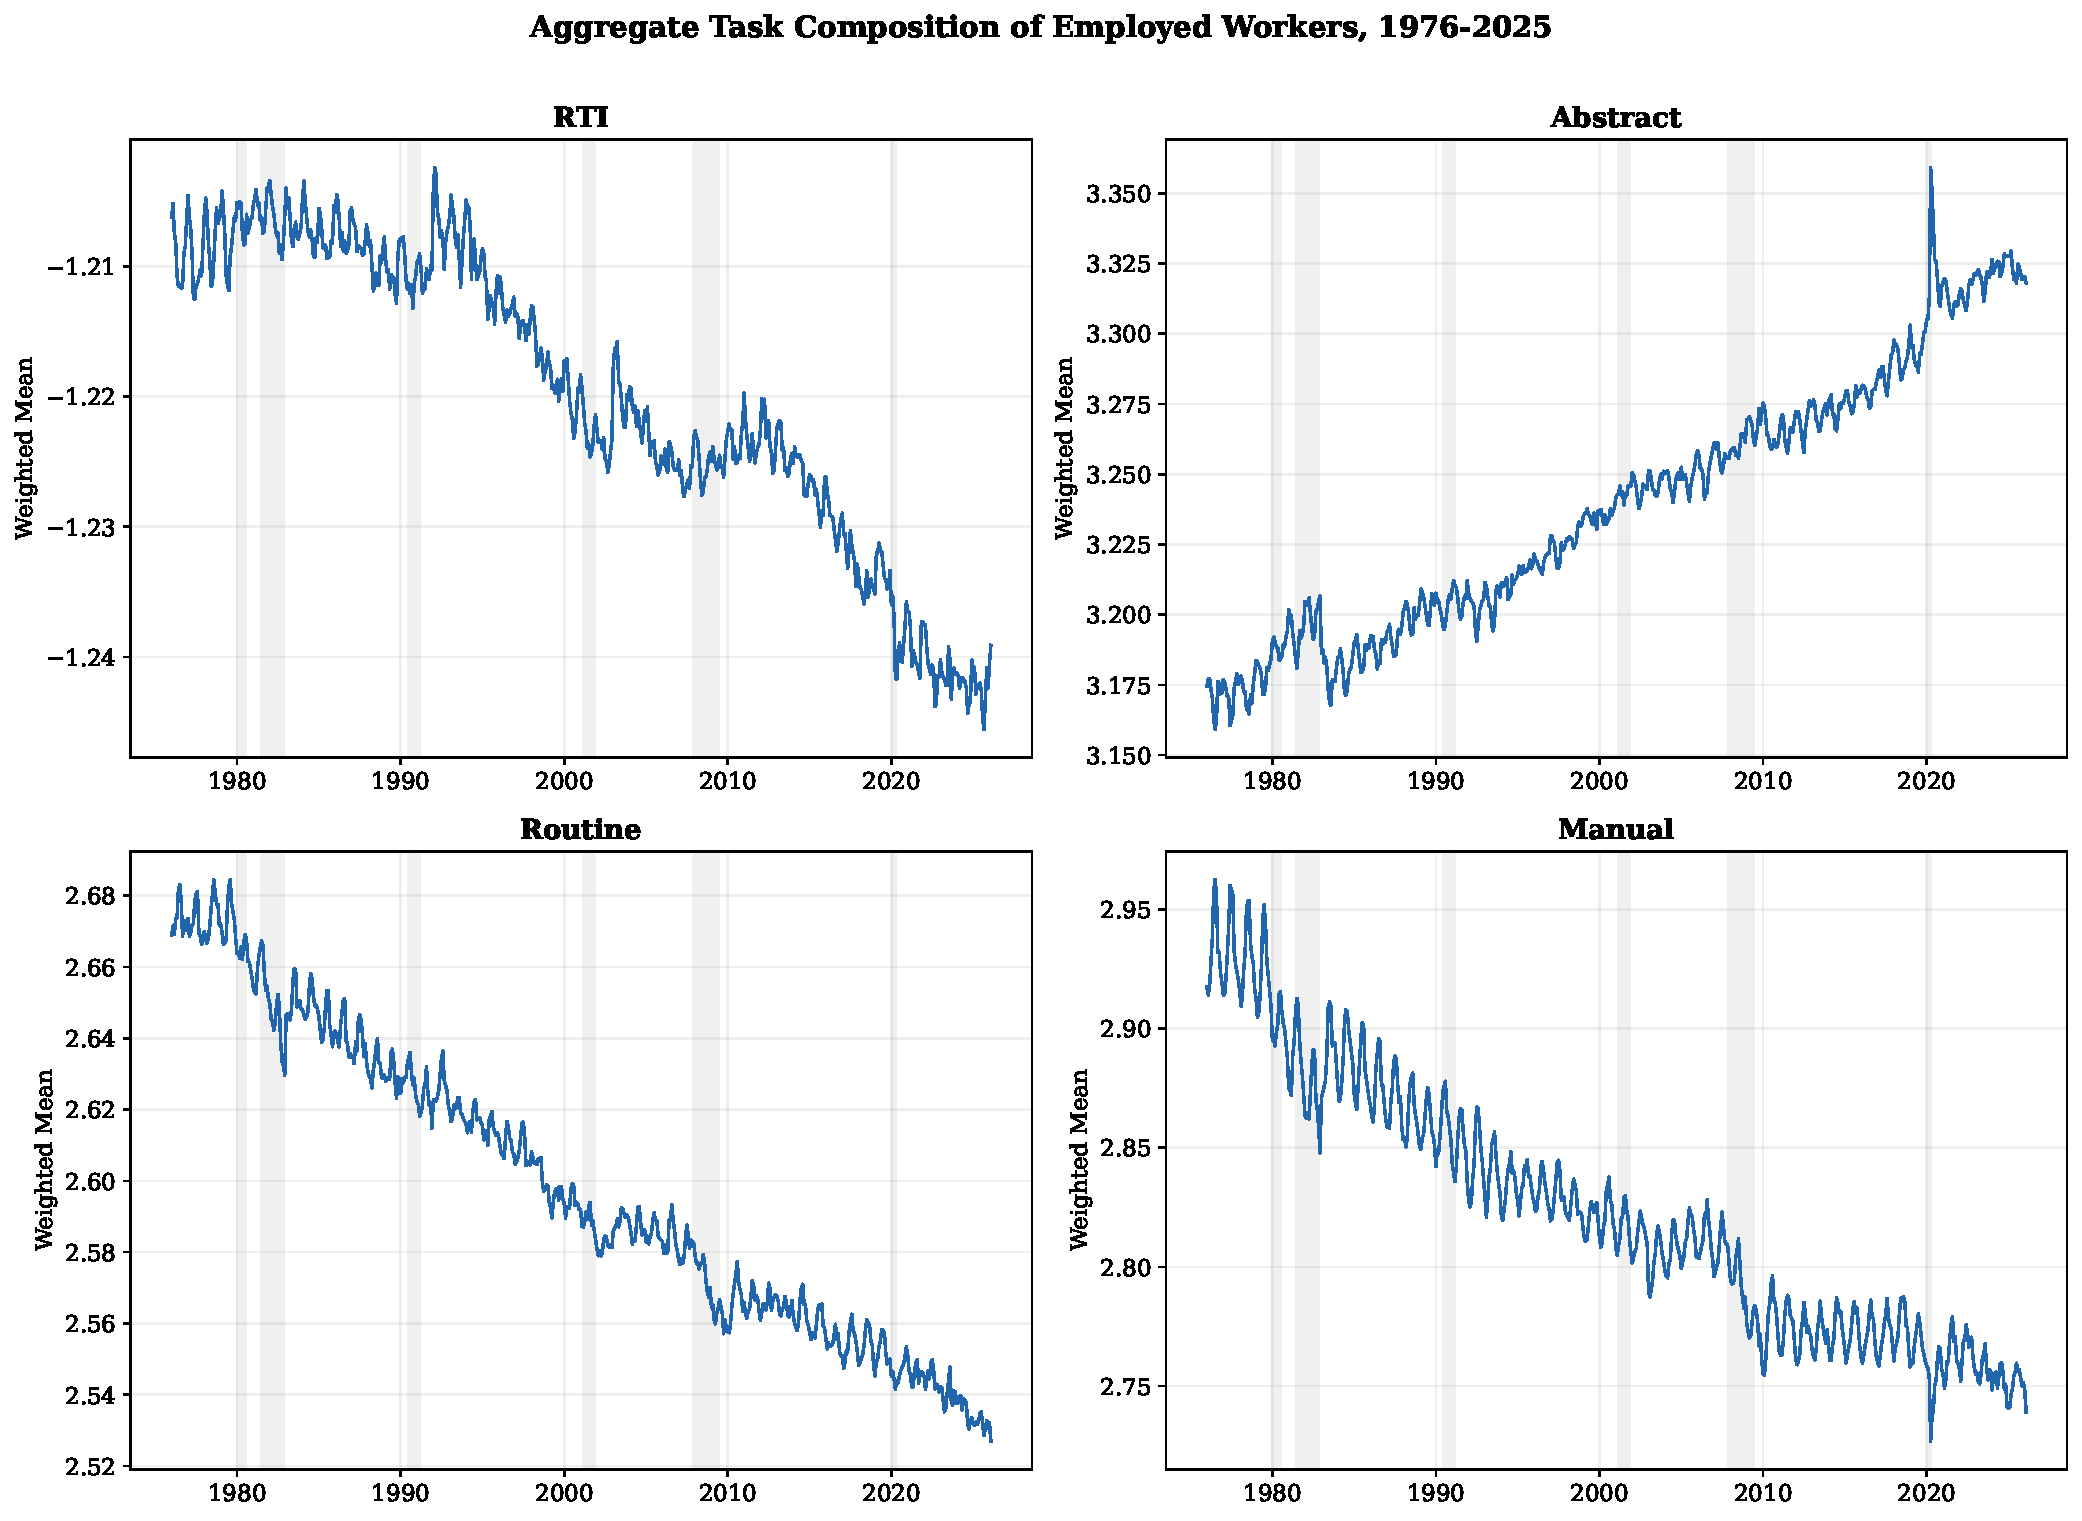
\includegraphics[width=\textwidth]{fig_timeseries.pdf}
	\caption{Aggregate Task Composition, \statsCpsStartYear--\statsYearMax. Gray shading: NBER recessions.}
	\label{fig:timeseries}
\end{figure}

\begin{figure}[htbp]
	\centering
	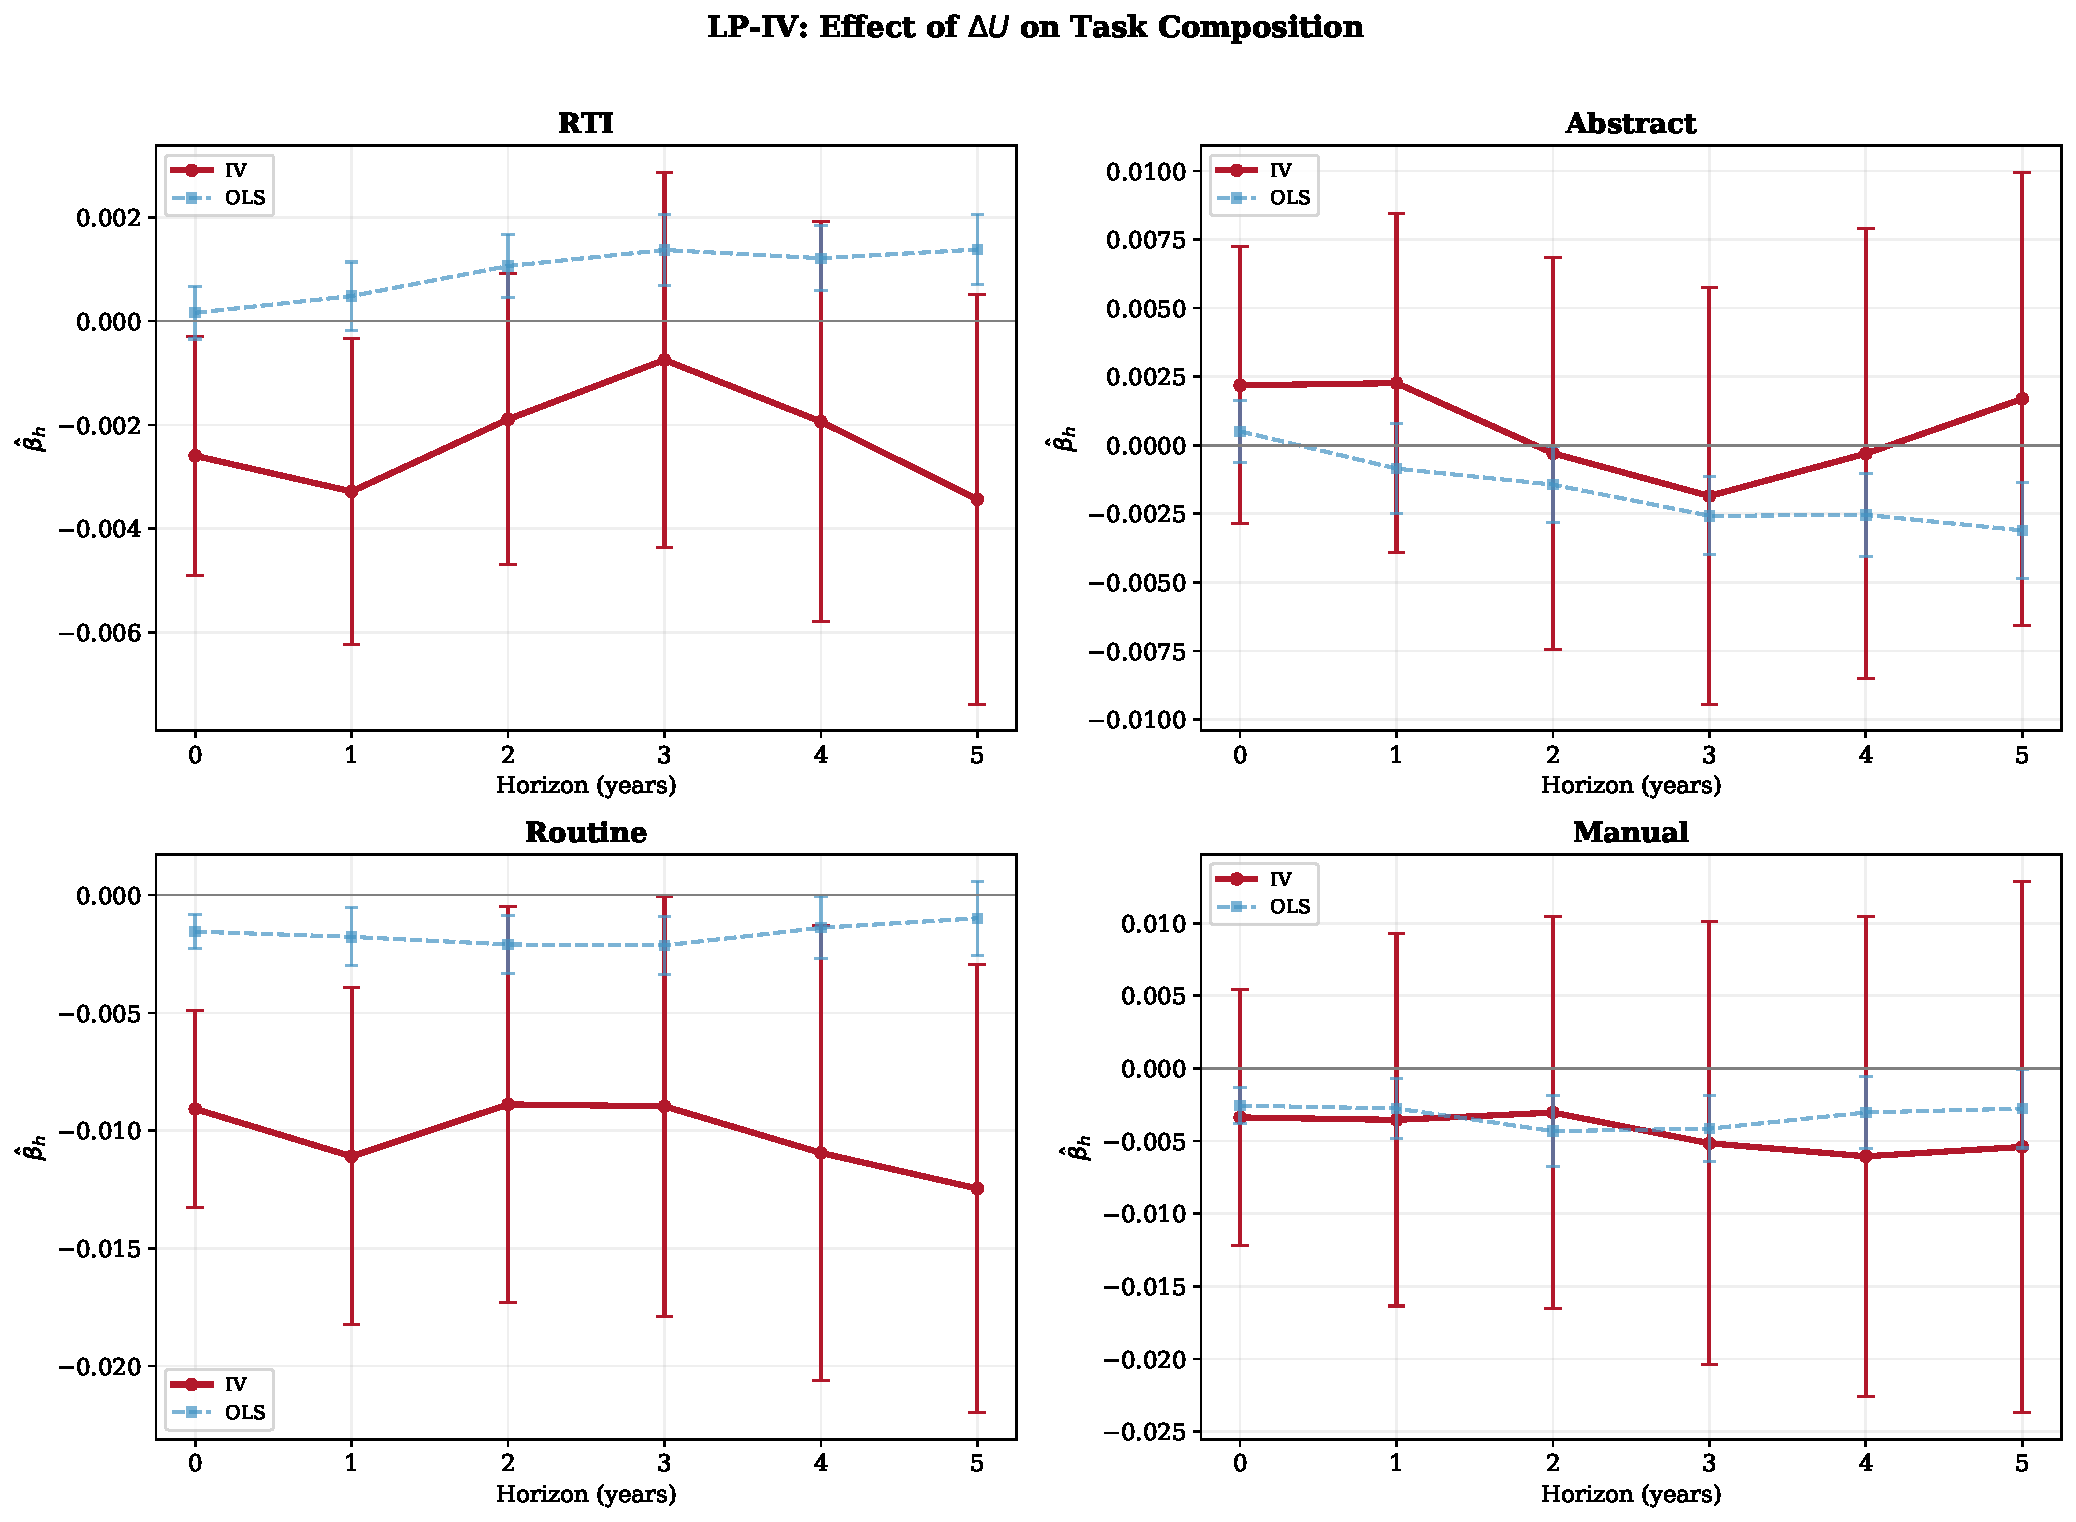
\includegraphics[width=\textwidth]{fig_lpiv_main.pdf}
	\caption{LP-IV Impulse Response. Red: IV (Bartik). Blue: OLS. Error bars: 95\% CI.}
	\label{fig:lpiv}
\end{figure}

\begin{figure}[htbp]
	\centering
	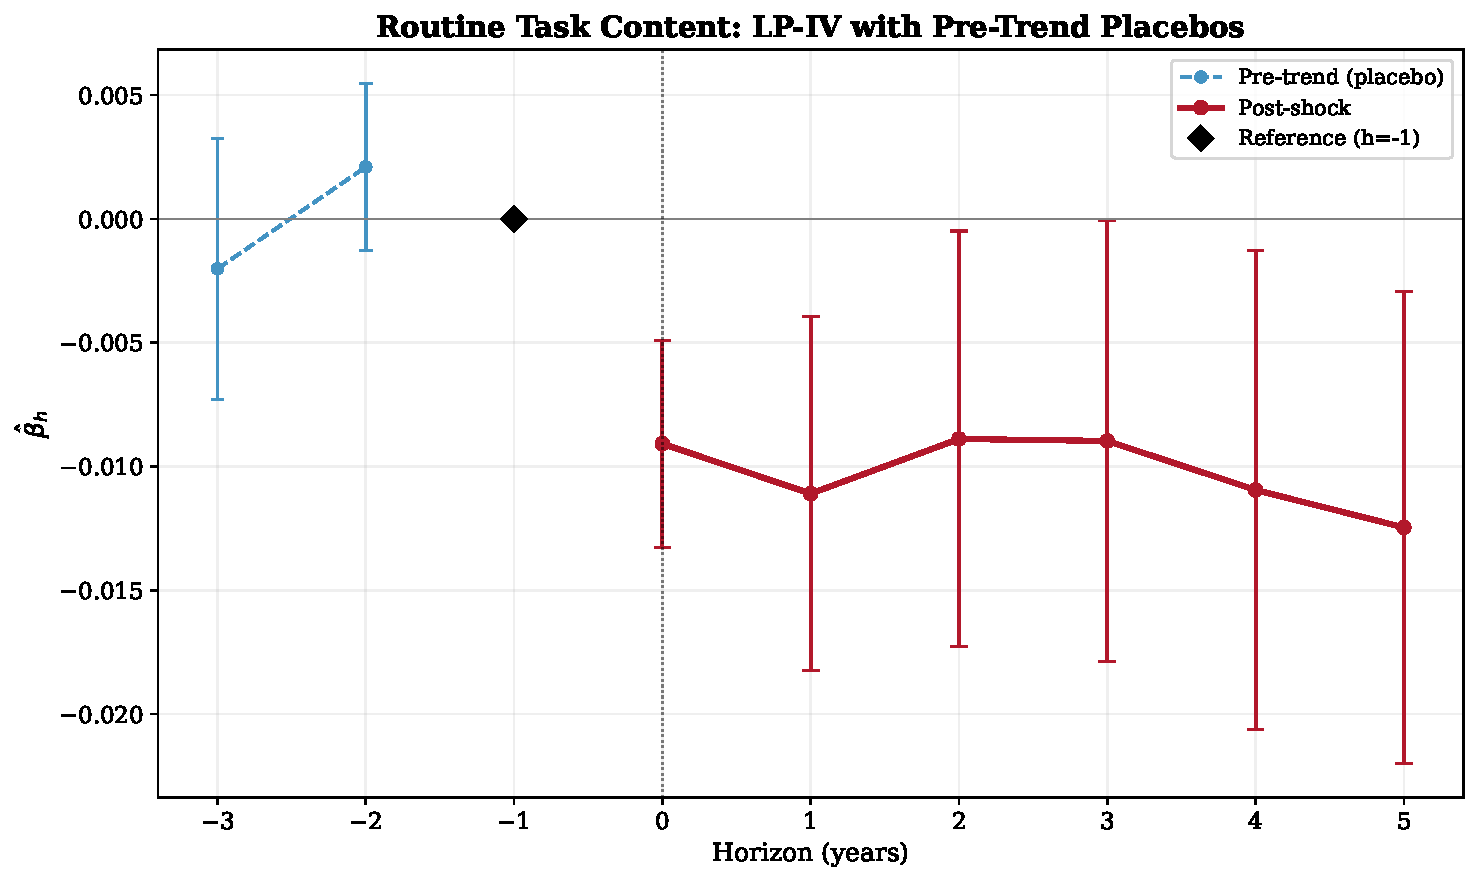
\includegraphics[width=0.85\textwidth]{fig_routine_pretrend.pdf}
	\caption{Routine: LP-IV with Pre-Trend Placebos. Clean pre-trends consistent with the identifying assumptions.}
	\label{fig:pretrend}
\end{figure}

\begin{figure}[htbp]
	\centering
	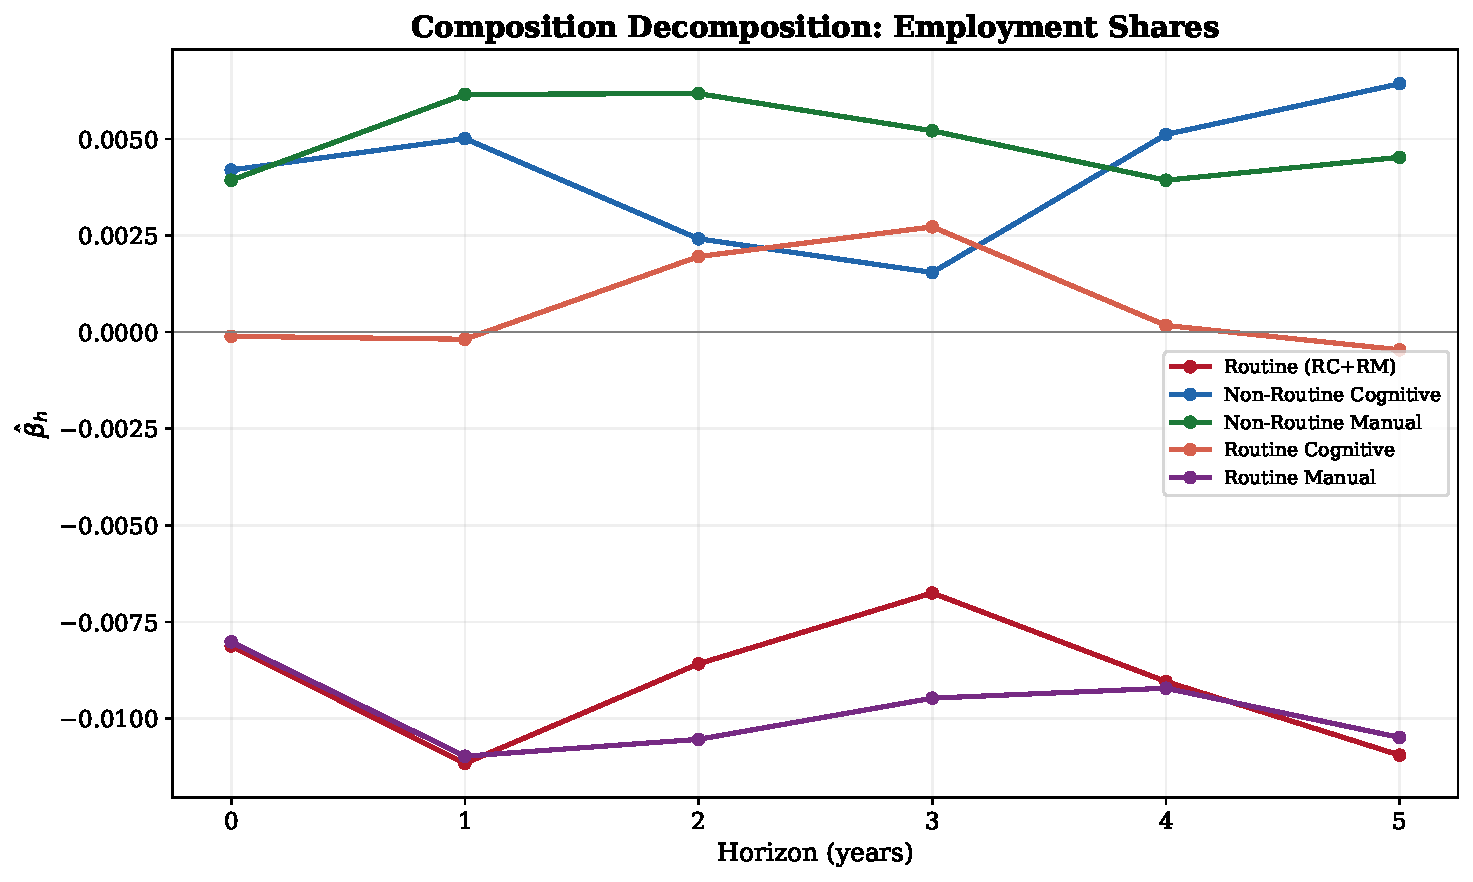
\includegraphics[width=0.85\textwidth]{fig_composition.pdf}
	\caption{Composition Decomposition. RM falls sharply; NRM rises by an offsetting amount.}
	\label{fig:composition}
\end{figure}

\begin{figure}[htbp]
	\centering
	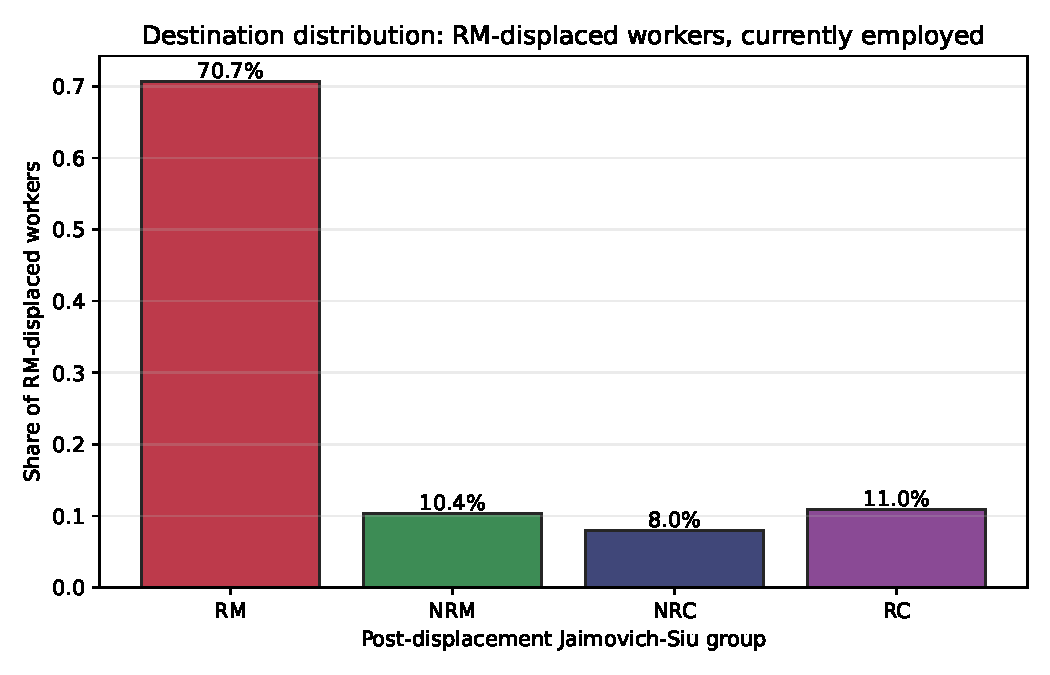
\includegraphics[width=0.75\textwidth]{fig_dws_destinations.pdf}
	\caption[DWS destinations]{Post-displacement destinations of routine-manual workers, Displaced Worker Survey supplements \statsDwsWaveMin--\statsDwsWaveMax. Sample: \statsDwsNObs{} workers aged 20--64 who involuntarily lost a full-time private-sector job in the previous 3--5 years and were currently employed at the time of the survey. Non-routine manual (service) and routine cognitive (sales / administrative support) are the two largest absorbing categories outside RM, at roughly equal shares; the rising NRM destination matches the persistent NRM share gain documented in the aggregate composition decomposition (Figure~\ref{fig:composition}, Table~\ref{tab:composition}).}
	\label{fig:dws_destinations}
\end{figure}

\begin{figure}[htbp]
	\centering
	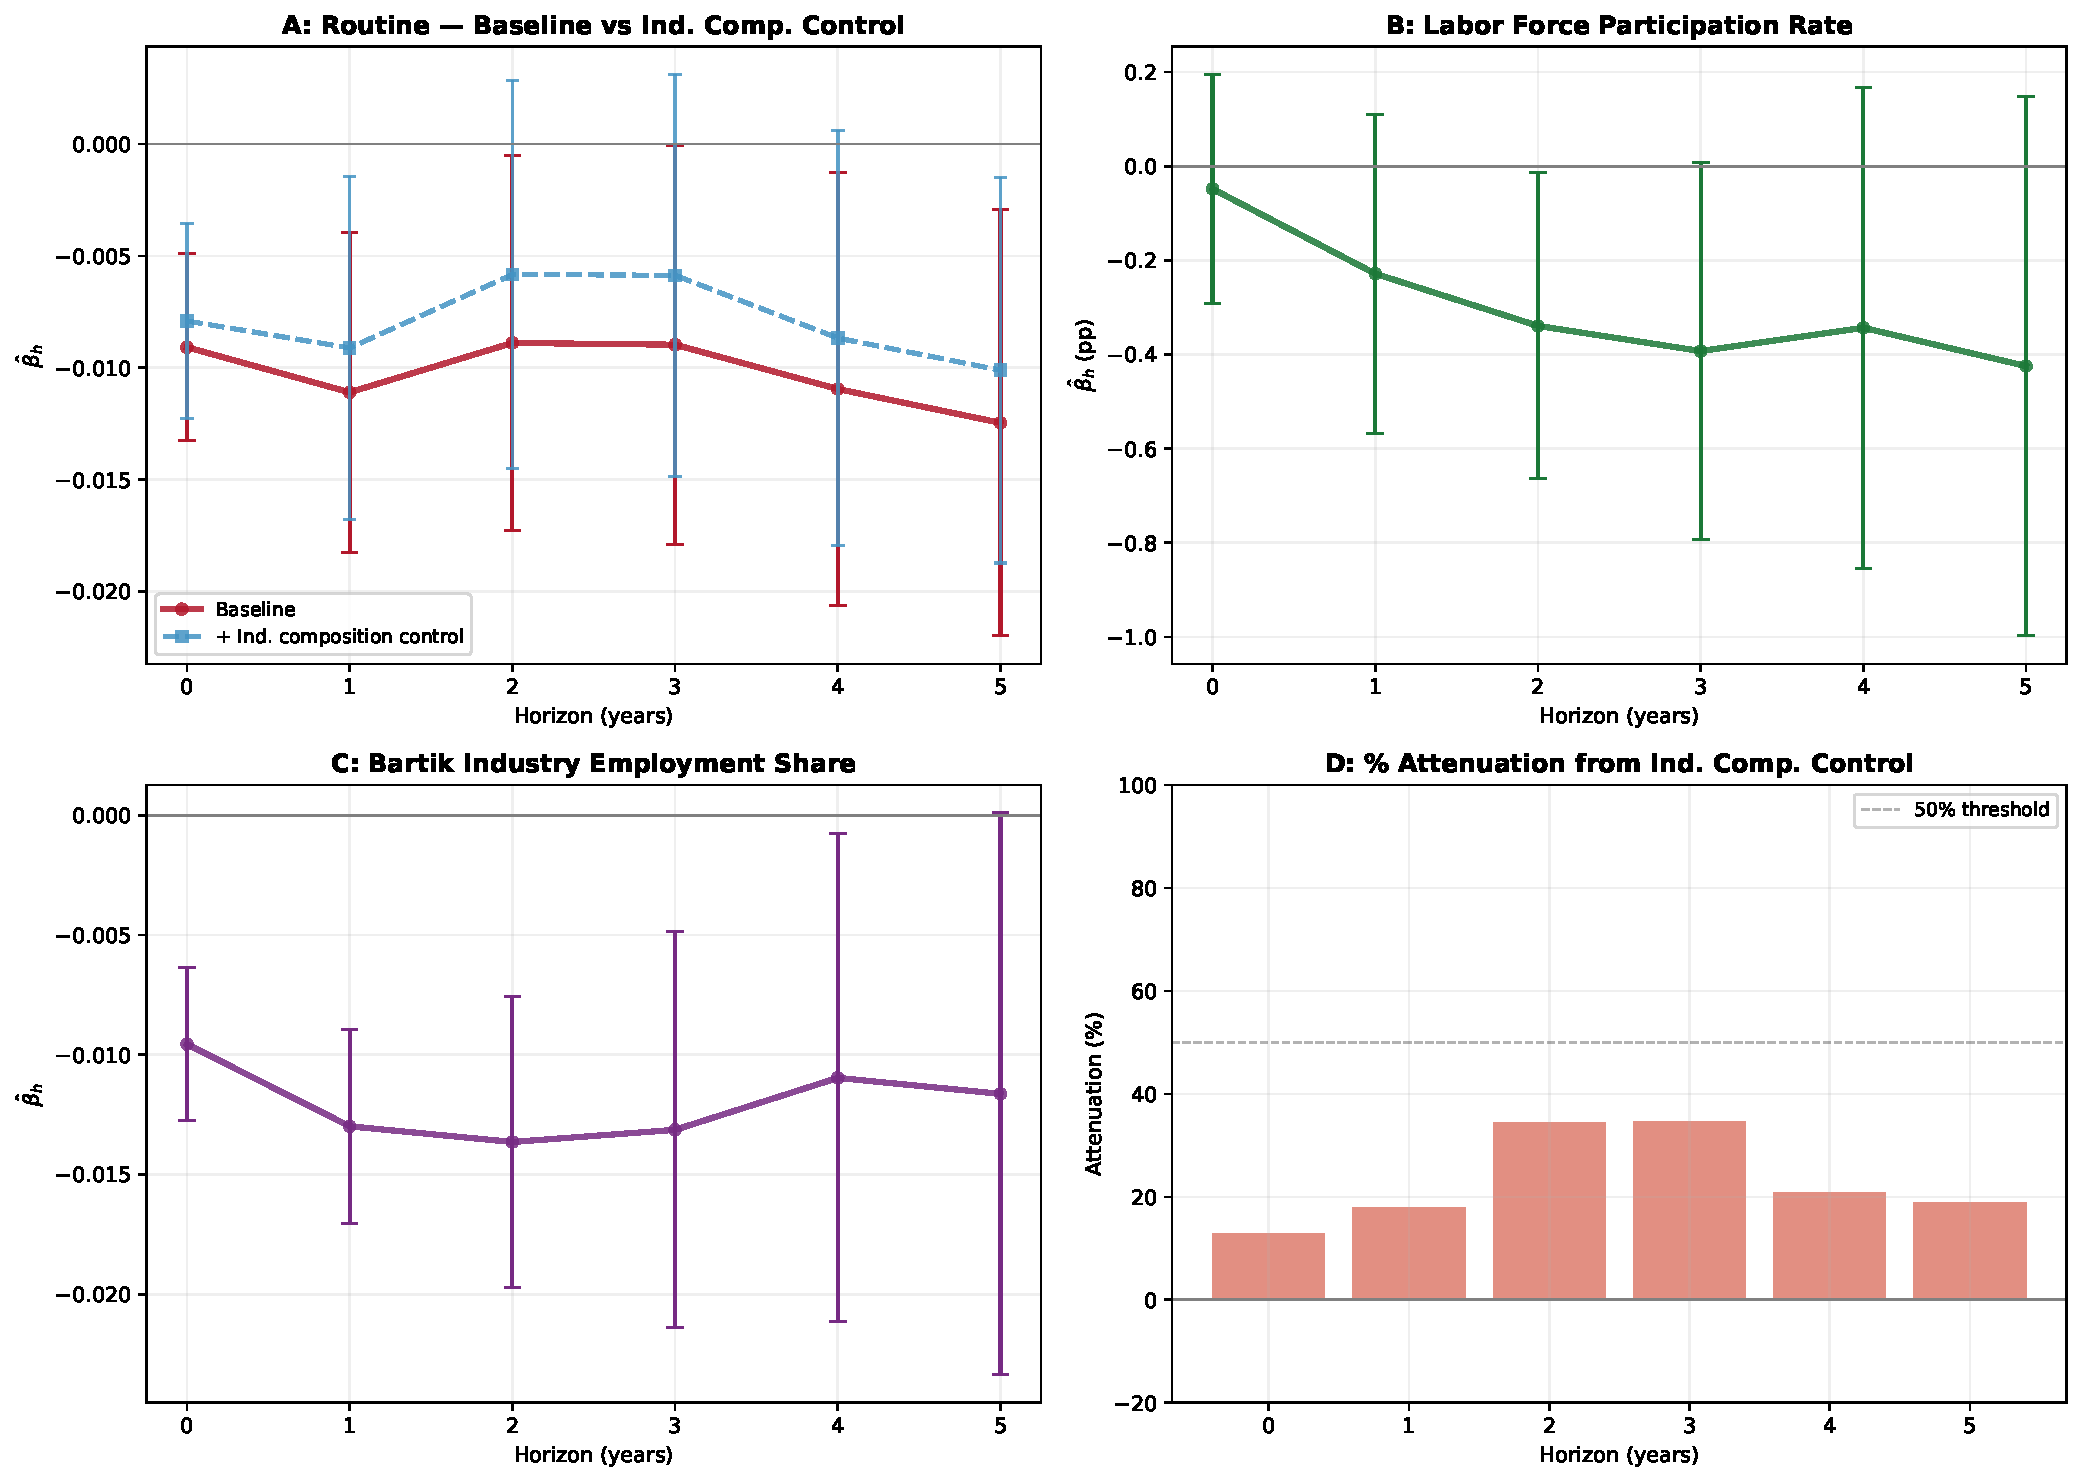
\includegraphics[width=0.85\textwidth]{../results/robustness/fig_mechanism_tests.pdf}
	\caption{Mechanism Test. (A) Baseline vs industry composition control: \statsMechAttenuationHzero\% attenuation at $h = 0$. (B) LFP response. (C) Bartik industry share response. (D) Attenuation by horizon.}
	\label{fig:mechanism}
\end{figure}


% ============================================================
% CRediT authorship contribution statement
% ============================================================
\printcredits


% ============================================================
\clearpage
\bibliographystyle{cas-model2-names}
\bibliography{references}


% ============================================================
% APPENDIX
% ============================================================
\clearpage
\appendix
\setcounter{table}{0}
\renewcommand{\thetable}{A\arabic{table}}
\setcounter{figure}{0}
\renewcommand{\thefigure}{A\arabic{figure}}

\section{Additional Results and Diagnostics}\label{sec:appendix}

\subsection{Instrument Diagnostics}

Table~\ref{tab:gpss} reports approximate Rotemberg weights. Identification is dispersed across cyclically sensitive industries. Table~\ref{tab:ar} reports Anderson-Rubin confidence sets: the 95\% CS for routine at $h = 0$ is [\statsArLower, \statsArUpper], excluding zero.

\begin{table}[htbp]
\centering
\caption{GPSS Rotemberg Weight Decomposition}
\label{tab:gpss}
\begin{tabular}{lccc}
\hline\hline
Industry & Avg. Emp. Share & SD(Nat. Growth) & Weight (\%) \\
\hline
Construction & 0.071 & 0.050 & 23.1 \\
Manufacturing - Durable goods & 0.084 & 0.038 & 16.2 \\
Professional and business services & 0.126 & 0.028 & 13.0 \\
Retail trade & 0.177 & 0.021 & 10.6 \\
Education and health services & 0.196 & 0.016 & 6.8 \\
Mining and logging & 0.010 & 0.070 & 6.5 \\
Transportation and warehousing & 0.046 & 0.028 & 4.7 \\
Leisure and hospitality & 0.018 & 0.040 & 3.8 \\
Other services & 0.039 & 0.026 & 3.5 \\
Manufacturing - Nondurable goods & 0.057 & 0.022 & 3.5 \\
Financial activities & 0.064 & 0.020 & 3.4 \\
Wholesale trade & 0.032 & 0.023 & 2.3 \\
Information & 0.012 & 0.033 & 1.8 \\
Government & 0.054 & 0.012 & 1.1 \\
\hline\hline
\end{tabular}
\begin{tablenotes}\small
\item Approximate Rotemberg weights following Goldsmith-Pinkham, Sorkin, and Swift (2020).
\end{tablenotes}
\end{table}
\begin{table}[htbp]
\centering
\caption{Weak-Instrument-Robust Inference: Anderson-Rubin Confidence Sets}
\label{tab:ar}
\begin{tabular}{lcc}
\hline\hline
& 2SLS & Anderson-Rubin \\
\hline
Point estimate & -0.0091 & --- \\
95\% CI & [-0.0133, -0.0049] & [-0.0136, -0.0052] \\
Excludes zero & Yes & Yes \\
\hline\hline
\end{tabular}
\begin{tablenotes}\small
\item AR confidence set constructed by inverting the Anderson-Rubin test over a grid of 400 values.
\end{tablenotes}
\end{table}

\subsection{Additional Robustness}

Table~\ref{tab:flex} replaces the linear technology control with initial routine share interacted with year fixed effects, a fully nonparametric absorption of state-specific secular technology trajectories. The first stage remains strong and the impact and $h = 1$ routine coefficients are similar in magnitude to the baseline, with persistence preserved. Table~\ref{tab:trends} adds state-specific linear trends to the baseline; point estimates are essentially unchanged. Table~\ref{tab:fixedbartik} replaces rolling pre-period industry shares with fixed initial-year (\statsBaseYear) shares, addressing the concern that the rolling base year could endogenously absorb medium-run reallocation. The impact estimate retains its sign and significance under fixed shares, but the effect attenuates sharply at longer horizons --- losing significance by $h = 1$ and changing sign at $h = 3$ and $h = 4$ --- as the predictive content of the \statsBaseYear{} industry composition decays over time.

\begin{table}[htbp]
\centering
\caption{Robustness: Flexible Technology Controls}
\label{tab:flex}
\begin{tabular}{lcc}
\hline\hline
Horizon $h$ & Baseline & Flexible Controls \\
\hline
0 & -0.0091$^{***}$ & -0.0099$^{***}$ \\
 & (0.0021) & (0.0025) \\[3pt]
1 & -0.0111$^{***}$ & -0.0148$^{***}$ \\
 & (0.0037) & (0.0044) \\[3pt]
2 & -0.0089$^{**}$ & -0.0128$^{**}$ \\
 & (0.0043) & (0.0057) \\[3pt]
3 & -0.0090$^{**}$ & -0.0128$^{**}$ \\
 & (0.0045) & (0.0058) \\[3pt]
4 & -0.0109$^{**}$ & -0.0162$^{***}$ \\
 & (0.0049) & (0.0058) \\[3pt]
5 & -0.0125$^{**}$ & -0.0189$^{***}$ \\
 & (0.0049) & (0.0061) \\[3pt]
\hline
Tech control & $\bar{\omega}^R_s \times t$ & $\bar{\omega}^R_s \times \theta_t$ \\
First-stage $F$ & {\statsFsF} & 17.4 \\
\hline\hline
\end{tabular}
\end{table}
\begin{table}[htbp]
\centering
\caption{Robustness: State-Specific Linear Trends}
\label{tab:trends}
\begin{tabular}{lcc}
\hline\hline
Horizon $h$ & Baseline & + State Trends \\
\hline
0 & -0.0091$^{***}$ & -0.0084$^{***}$ \\
 & (0.0021) & (0.0020) \\[3pt]
1 & -0.0111$^{***}$ & -0.0101$^{***}$ \\
 & (0.0037) & (0.0035) \\[3pt]
2 & -0.0089$^{**}$ & -0.0075$^{*}$ \\
 & (0.0043) & (0.0041) \\[3pt]
3 & -0.0090$^{**}$ & -0.0069$^{*}$ \\
 & (0.0045) & (0.0041) \\[3pt]
4 & -0.0109$^{**}$ & -0.0076$^{*}$ \\
 & (0.0049) & (0.0043) \\[3pt]
5 & -0.0125$^{**}$ & -0.0079$^{**}$ \\
 & (0.0049) & (0.0040) \\[3pt]
\hline\hline
\end{tabular}
\end{table}
\begin{table}[htbp]
\centering
\caption{Robustness: Fixed Base-Year ({\statsBaseYear}) Bartik Shares}
\label{tab:fixedbartik}
\begin{tabular}{lcc}
\hline\hline
Horizon $h$ & Rolling Shares & Fixed {\statsBaseYear} Shares \\
\hline
0 & -0.0091$^{***}$ & -0.0064$^{***}$ \\
 & (0.0021) & (0.0020) \\[3pt]
1 & -0.0111$^{***}$ & -0.0056 \\
 & (0.0037) & (0.0040) \\[3pt]
2 & -0.0089$^{**}$ & -0.0002 \\
 & (0.0043) & (0.0044) \\[3pt]
3 & -0.0090$^{**}$ & 0.0025 \\
 & (0.0045) & (0.0058) \\[3pt]
4 & -0.0109$^{**}$ & 0.0008 \\
 & (0.0049) & (0.0065) \\[3pt]
5 & -0.0125$^{**}$ & -0.0012 \\
 & (0.0049) & (0.0059) \\[3pt]
\hline
First-stage $F$ & {\statsFsF} & 14.9 \\
\hline\hline
\end{tabular}
\end{table}

\subsection{Labor Force Participation}

Table~\ref{tab:lfp} estimates the LP-IV with the state labor force participation rate as the outcome. The impact effect ($\hat\beta_0 = \statsLfpHzeroBeta$ percentage points per one-percentage-point unemployment increase) is statistically indistinguishable from zero. The LFP response remains small at all horizons relative to the task-composition effect, ruling out differential labor force exit as a driver of the headline result. See Section~\ref{sec:selection} for the main-text discussion.

\begin{table}[htbp]
\centering
\caption{Selection Test: Effect on Labor Force Participation Rate}
\label{tab:lfp}
\begin{tabular}{lc}
\hline\hline
Horizon $h$ & $\Delta$ LFP Rate (pp) \\
\hline
0 & -0.0483 \\
 & (0.1242) \\[3pt]
1 & -0.2284 \\
 & (0.1730) \\[3pt]
2 & -0.3392$^{**}$ \\
 & (0.1658) \\[3pt]
3 & -0.3928$^{*}$ \\
 & (0.2042) \\[3pt]
4 & -0.3433 \\
 & (0.2606) \\[3pt]
5 & -0.4246 \\
 & (0.2925) \\[3pt]
\hline\hline
\end{tabular}
\begin{tablenotes}\small
\item Same LP-IV specification as the main results.
\item A 1 pp increase in unemployment changes the LFP rate by -0.0483 pp at impact, statistically indistinguishable from zero.
\end{tablenotes}
\end{table}

\subsection{Robustness Summary}

Figure~\ref{fig:robustness_app} compares the routine impulse response across the baseline, flexible technology controls, and state-specific trend specifications. All three produce similar impact effects and similar persistent dynamics through the five-year horizon.

\begin{figure}[htbp]
	\centering
	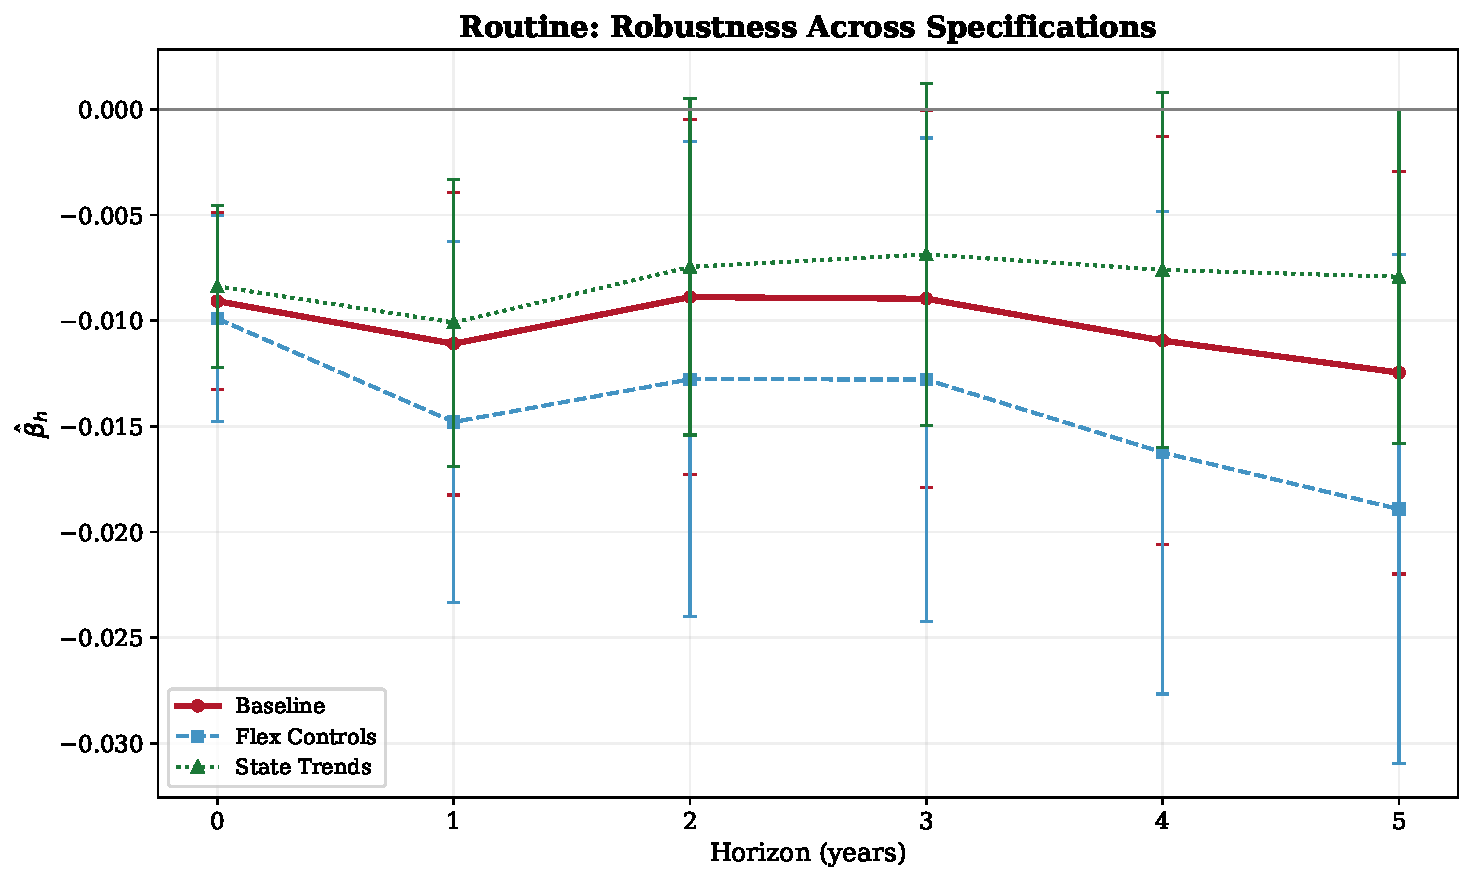
\includegraphics[width=0.85\textwidth]{fig_robustness.pdf}
	\caption{Routine LP-IV across specifications. Baseline (red), flexible controls (blue), state trends (green).}
	\label{fig:robustness_app}
\end{figure}

\subsection{Leave-One-Industry-Out Bartik}

Table~\ref{tab:loo} re-estimates the LP-IV after dropping each of the top three Rotemberg-weight industries from the Bartik instrument and renormalizing the remaining shares. The routine impact response retains its sign, magnitude, and statistical significance under all three exclusions. No single industry is necessary for identification: the result is supported by demand variation arising in construction, durable manufacturing, professional and business services, and retail trade, the four leading cyclical industries by Rotemberg weight.

\begin{table}[htbp]
\centering
\caption{Leave-One-Industry-Out Bartik: Routine Task Content}
\label{tab:loo}
\small
\resizebox{\textwidth}{!}{\begin{tabular}{lcccc}
\hline\hline
Horizon & Baseline & Drop Construction & Drop Manufacturing - Durable goods & Drop Professional and business services \\
\hline
0 & -0.0091$^{***}$ & -0.0077$^{***}$ & -0.0064$^{***}$ & -0.0076$^{***}$ \\
 & (0.0021) & (0.0015) & (0.0016) & (0.0018) \\[3pt]
1 & -0.0111$^{***}$ & -0.0089$^{***}$ & -0.0083$^{***}$ & -0.0082$^{**}$ \\
 & (0.0037) & (0.0024) & (0.0025) & (0.0036) \\[3pt]
2 & -0.0089$^{**}$ & -0.0066$^{**}$ & -0.0058$^{*}$ & -0.0050 \\
 & (0.0043) & (0.0029) & (0.0031) & (0.0040) \\[3pt]
3 & -0.0090$^{**}$ & -0.0069$^{**}$ & -0.0055 & -0.0046 \\
 & (0.0045) & (0.0032) & (0.0036) & (0.0044) \\[3pt]
4 & -0.0109$^{**}$ & -0.0078$^{**}$ & -0.0066$^{*}$ & -0.0057 \\
 & (0.0049) & (0.0038) & (0.0039) & (0.0050) \\[3pt]
5 & -0.0125$^{**}$ & -0.0079$^{**}$ & -0.0071$^{*}$ & -0.0068 \\
 & (0.0049) & (0.0039) & (0.0037) & (0.0048) \\[3pt]
\hline
First-stage $F$ & {\statsFsF} & 34.9 & 20.7 & 23.0 \\
\hline\hline
\end{tabular}}
\begin{tablenotes}\small
\item Each column drops the named industry from the Bartik instrument and renormalizes shares.
\item $^{***}p<0.01$, $^{**}p<0.05$, $^{*}p<0.1$.
\end{tablenotes}
\end{table}

\subsection{Heterogeneity by Routine Intensity}

Table~\ref{tab:routine_split} reports the LP-IV separately for states above and below the median initial (\statsBaseYear) routine employment share. The main discussion of these estimates is in Section~\ref{sec:results}; the table is reproduced here for completeness and to display the full coefficient set across all horizons for both subsamples.

\begin{table}[htbp]
\centering
\caption{Heterogeneity by Initial Routine Intensity}
\label{tab:routine_split}
\begin{tabular}{lcc}
\hline\hline
Horizon & High Routine & Low Routine \\
\hline
0 & -0.0098$^{**}$ & -0.0089$^{***}$ \\
 & (0.0042) & (0.0031) \\[3pt]
1 & -0.0120$^{*}$ & -0.0124$^{**}$ \\
 & (0.0064) & (0.0051) \\[3pt]
2 & -0.0077 & -0.0121$^{**}$ \\
 & (0.0083) & (0.0051) \\[3pt]
3 & -0.0101 & -0.0111$^{**}$ \\
 & (0.0089) & (0.0055) \\[3pt]
4 & -0.0156$^{*}$ & -0.0110$^{**}$ \\
 & (0.0093) & (0.0056) \\[3pt]
5 & -0.0210$^{**}$ & -0.0110$^{**}$ \\
 & (0.0097) & (0.0054) \\[3pt]
\hline\hline
\end{tabular}
\begin{tablenotes}\small
\item States split at median initial ({\statsBaseYear}) routine employment share.
\end{tablenotes}
\end{table}

\subsection{Occupation-Type Heterogeneity}

Table~\ref{tab:educ} estimates the LP-IV separately for college-type and non-college-type occupations. The entire effect is concentrated in non-college occupations, where routine manual workers are predominantly employed.

\begin{table}[htbp]
\centering
\caption{Occupation-Type Heterogeneity: Routine Task Content}
\label{tab:educ}
\begin{tabular}{lcc}
\hline\hline
Horizon & College-Type Occ. & Non-College-Type Occ. \\
\hline
0 & 0.0015 & -0.0113$^{***}$ \\
 & (0.0016) & (0.0026) \\[3pt]
1 & 0.0032 & -0.0156$^{***}$ \\
 & (0.0032) & (0.0033) \\[3pt]
2 & 0.0057 & -0.0153$^{***}$ \\
 & (0.0042) & (0.0035) \\[3pt]
3 & 0.0037 & -0.0142$^{***}$ \\
 & (0.0035) & (0.0039) \\[3pt]
4 & 0.0029 & -0.0138$^{***}$ \\
 & (0.0036) & (0.0045) \\[3pt]
5 & 0.0060 & -0.0155$^{***}$ \\
 & (0.0052) & (0.0044) \\[3pt]
\hline\hline
\end{tabular}
\begin{tablenotes}\small
\item College-type: OCC2010 $<$ 3600 (management, professional, technical).
\item Non-college-type: OCC2010 $\geq$ 3600 (service, production, operators).
\item $^{***}p<0.01$, $^{**}p<0.05$, $^{*}p<0.1$.
\end{tablenotes}
\end{table}

\subsection{Age Group Heterogeneity}

Table~\ref{tab:age} reveals that young workers experience the largest immediate displacement and the most persistent response, prime-age workers show a smaller effect that is significant at impact and at $h = 5$ but not at the intermediate horizons, and older workers exhibit a delayed response that peaks at intermediate horizons.

\begin{table}[htbp]
\centering
\caption{Age Group Heterogeneity: Routine Task Content}
\label{tab:age}
\begin{tabular}{lccc}
\hline\hline
Horizon & Young (16-29) & Prime Age (30-54) & Older (55+) \\
\hline
0 & -0.0147$^{***}$ & -0.0071$^{***}$ & -0.0043 \\
 & (0.0032) & (0.0025) & (0.0034) \\[3pt]
1 & -0.0148$^{***}$ & -0.0086$^{**}$ & -0.0099$^{*}$ \\
 & (0.0047) & (0.0042) & (0.0051) \\[3pt]
2 & -0.0084 & -0.0065 & -0.0140$^{***}$ \\
 & (0.0059) & (0.0051) & (0.0048) \\[3pt]
3 & -0.0113$^{*}$ & -0.0052 & -0.0124$^{**}$ \\
 & (0.0064) & (0.0052) & (0.0061) \\[3pt]
4 & -0.0115$^{**}$ & -0.0087 & -0.0121 \\
 & (0.0057) & (0.0056) & (0.0077) \\[3pt]
5 & -0.0135$^{**}$ & -0.0107$^{**}$ & -0.0093 \\
 & (0.0064) & (0.0052) & (0.0078) \\[3pt]
\hline\hline
\end{tabular}
\end{table}

\subsection{Alternative Treatment Variable}

Table~\ref{tab:empgrowth} replaces $\Delta U_{st}$ with $\Delta \log(\text{emp})_{st}$ as the endogenous variable. Significant effects at $h = 0$ and $h = 1$ confirm the result is not specific to the unemployment measure.

\begin{table}[htbp]
\centering
\caption{Alternative Treatment: $\Delta U$ vs $\Delta \log(\text{emp})$}
\label{tab:empgrowth}
\begin{tabular}{lcc}
\hline\hline
Horizon & $\Delta U$ (baseline) & $\Delta \log(\text{emp})$ \\
\hline
0 & -0.0091$^{***}$ & 0.6954$^{**}$ \\
 & (0.0021) & (0.3428) \\[3pt]
1 & -0.0111$^{***}$ & 0.8447$^{*}$ \\
 & (0.0037) & (0.4645) \\[3pt]
2 & -0.0089$^{**}$ & 0.6764 \\
 & (0.0043) & (0.4944) \\[3pt]
3 & -0.0090$^{**}$ & 0.6758 \\
 & (0.0045) & (0.4899) \\[3pt]
4 & -0.0109$^{**}$ & 0.8309 \\
 & (0.0049) & (0.5137) \\[3pt]
5 & -0.0125$^{**}$ & 0.9233$^{*}$ \\
 & (0.0049) & (0.4803) \\[3pt]
\hline
First-stage $F$ & 23.3 & 5.7 \\
\hline\hline
\end{tabular}
\begin{tablenotes}\small
\item Coefficients have different scales: $\Delta U$ is per 1pp unemployment increase;
$\Delta \log(\text{emp})$ is per 1\% employment change.
\end{tablenotes}
\end{table}

\subsection{Census Region by Year Trends}

Table~\ref{tab:region} adds census region $\times$ year fixed effects to absorb broad regional business cycles. The first stage remains strong, and the routine impulse response is essentially unchanged in magnitude at every horizon, with significance preserved at impact, $h = 1$, $h = 2$, and $h = 5$. At $h = 3$ and $h = 4$ the controlled estimate retains the baseline sign and a similar point magnitude but loses statistical significance under the more demanding region-by-year specification, consistent with part of the cyclically sensitive variation that identifies $\beta_h$ being absorbed by region-specific business cycles at those horizons. The headline conclusion --- that the result is not driven by differential trends across census regions --- holds with this caveat.

\begin{table}[htbp]
\centering
\caption{Robustness: Census Region $\times$ Year Trends}
\label{tab:region}
\begin{tabular}{lcc}
\hline\hline
Horizon & Baseline & + Region $\times$ Year \\
\hline
0 & -0.0091$^{***}$ & -0.0086$^{***}$ \\
 & (0.0021) & (0.0020) \\[3pt]
1 & -0.0111$^{***}$ & -0.0100$^{***}$ \\
 & (0.0037) & (0.0037) \\[3pt]
2 & -0.0089$^{**}$ & -0.0068$^{*}$ \\
 & (0.0043) & (0.0041) \\[3pt]
3 & -0.0090$^{**}$ & -0.0066 \\
 & (0.0045) & (0.0045) \\[3pt]
4 & -0.0109$^{**}$ & -0.0079 \\
 & (0.0049) & (0.0050) \\[3pt]
5 & -0.0125$^{**}$ & -0.0097$^{**}$ \\
 & (0.0049) & (0.0048) \\[3pt]
\hline
First-stage $F$ & {\statsFsF} & 21.3 \\
\hline\hline
\end{tabular}
\end{table}

\subsection{Sample-Period Robustness}

Table~\ref{tab:robustness} reports the routine LP-IV across the baseline and five alternative specifications: flexible technology controls, state-specific trends, a pre-2008 sample, a post-2008 sample, and dropping the 2020--21 COVID episode. The impact effect is preserved across all five specifications. Excluding 2020--21 leaves the headline pattern essentially unchanged, with significance preserved at every horizon through $h = 5$, confirming that the COVID episode is not driving the result. The pre-2008 and post-2008 splits both deliver a significant impact effect of similar magnitude to the baseline. The pre-2008 long-horizon estimates remain negative and of similar magnitude to the full-sample baseline but lose statistical significance at $h = 3$ through $h = 5$ as standard errors widen in the smaller subsample. The post-2008 sample is qualitatively different: the impact effect is preserved, but the longer-horizon point estimates collapse toward zero and briefly turn weakly positive at $h = 3$, indicating that the persistence finding is identified primarily from the pre-2008 portion of the sample. The full-sample persistence result therefore does not survive an isolated post-2008 estimation; the impact effect, which is the load-bearing identification in the paper, does.

\begin{table}[htbp]
\centering
\caption{Robustness: LP-IV for Routine Task Content}
\label{tab:robustness}
\small
\begin{tabular}{lcccccc}
\hline\hline
Horizon & Baseline & Flex. Tech Controls & State Trends & Pre-2008 & Post-2008 & Drop 2020-21 \\
\hline
0 & -0.0091$^{***}$ & -0.0099$^{***}$ & -0.0084$^{***}$ & -0.0085$^{***}$ & -0.0082$^{**}$ & -0.0095$^{***}$ \\
 & (0.0021) & (0.0025) & (0.0020) & (0.0031) & (0.0034) & (0.0028) \\[3pt]
1 & -0.0111$^{***}$ & -0.0148$^{***}$ & -0.0101$^{***}$ & -0.0122$^{**}$ & -0.0058 & -0.0120$^{**}$ \\
 & (0.0037) & (0.0044) & (0.0035) & (0.0051) & (0.0046) & (0.0048) \\[3pt]
2 & -0.0089$^{**}$ & -0.0128$^{**}$ & -0.0075$^{*}$ & -0.0122$^{**}$ & -0.0002 & -0.0108$^{*}$ \\
 & (0.0043) & (0.0057) & (0.0041) & (0.0062) & (0.0039) & (0.0056) \\[3pt]
3 & -0.0090$^{**}$ & -0.0128$^{**}$ & -0.0069$^{*}$ & -0.0103 & 0.0010 & -0.0110$^{**}$ \\
 & (0.0045) & (0.0058) & (0.0041) & (0.0064) & (0.0033) & (0.0056) \\[3pt]
4 & -0.0109$^{**}$ & -0.0162$^{***}$ & -0.0076$^{*}$ & -0.0111 & -0.0004 & -0.0117$^{*}$ \\
 & (0.0049) & (0.0058) & (0.0043) & (0.0073) & (0.0035) & (0.0064) \\[3pt]
5 & -0.0125$^{**}$ & -0.0189$^{***}$ & -0.0079$^{**}$ & -0.0071 & -0.0045 & -0.0097$^{*}$ \\
 & (0.0049) & (0.0061) & (0.0040) & (0.0069) & (0.0050) & (0.0058) \\[3pt]
\hline\hline
\end{tabular}
\begin{tablenotes}\small
\item All specifications instrument $\Delta U_{st}$ with Bartik shift-share.
\item $^{***}p<0.01$, $^{**}p<0.05$, $^{*}p<0.1$.
\end{tablenotes}
\end{table}

\subsection{Extension Figures}

Figures~\ref{fig:extensions} and~\ref{fig:final_extensions} display the LP-IV impulse responses for the robustness and heterogeneity exercises tabulated above. Figure~\ref{fig:extensions} plots the leave-one-industry-out Bartik variants, the occupation-type split, and the census region $\times$ year specification (Appendix Tables~\ref{tab:loo}, \ref{tab:educ}, and~\ref{tab:region}). Figure~\ref{fig:final_extensions} plots the alternative treatment variable, the high- versus low-routine-state split, and the age-group decomposition (Appendix Tables~\ref{tab:empgrowth}, \ref{tab:routine_split}, and~\ref{tab:age}). The visual patterns mirror the coefficient tables: the impact effect is preserved across every alternative specification and across every subsample, and the long-horizon point estimates remain negative in every variant.

\begin{figure}[htbp]
	\centering
	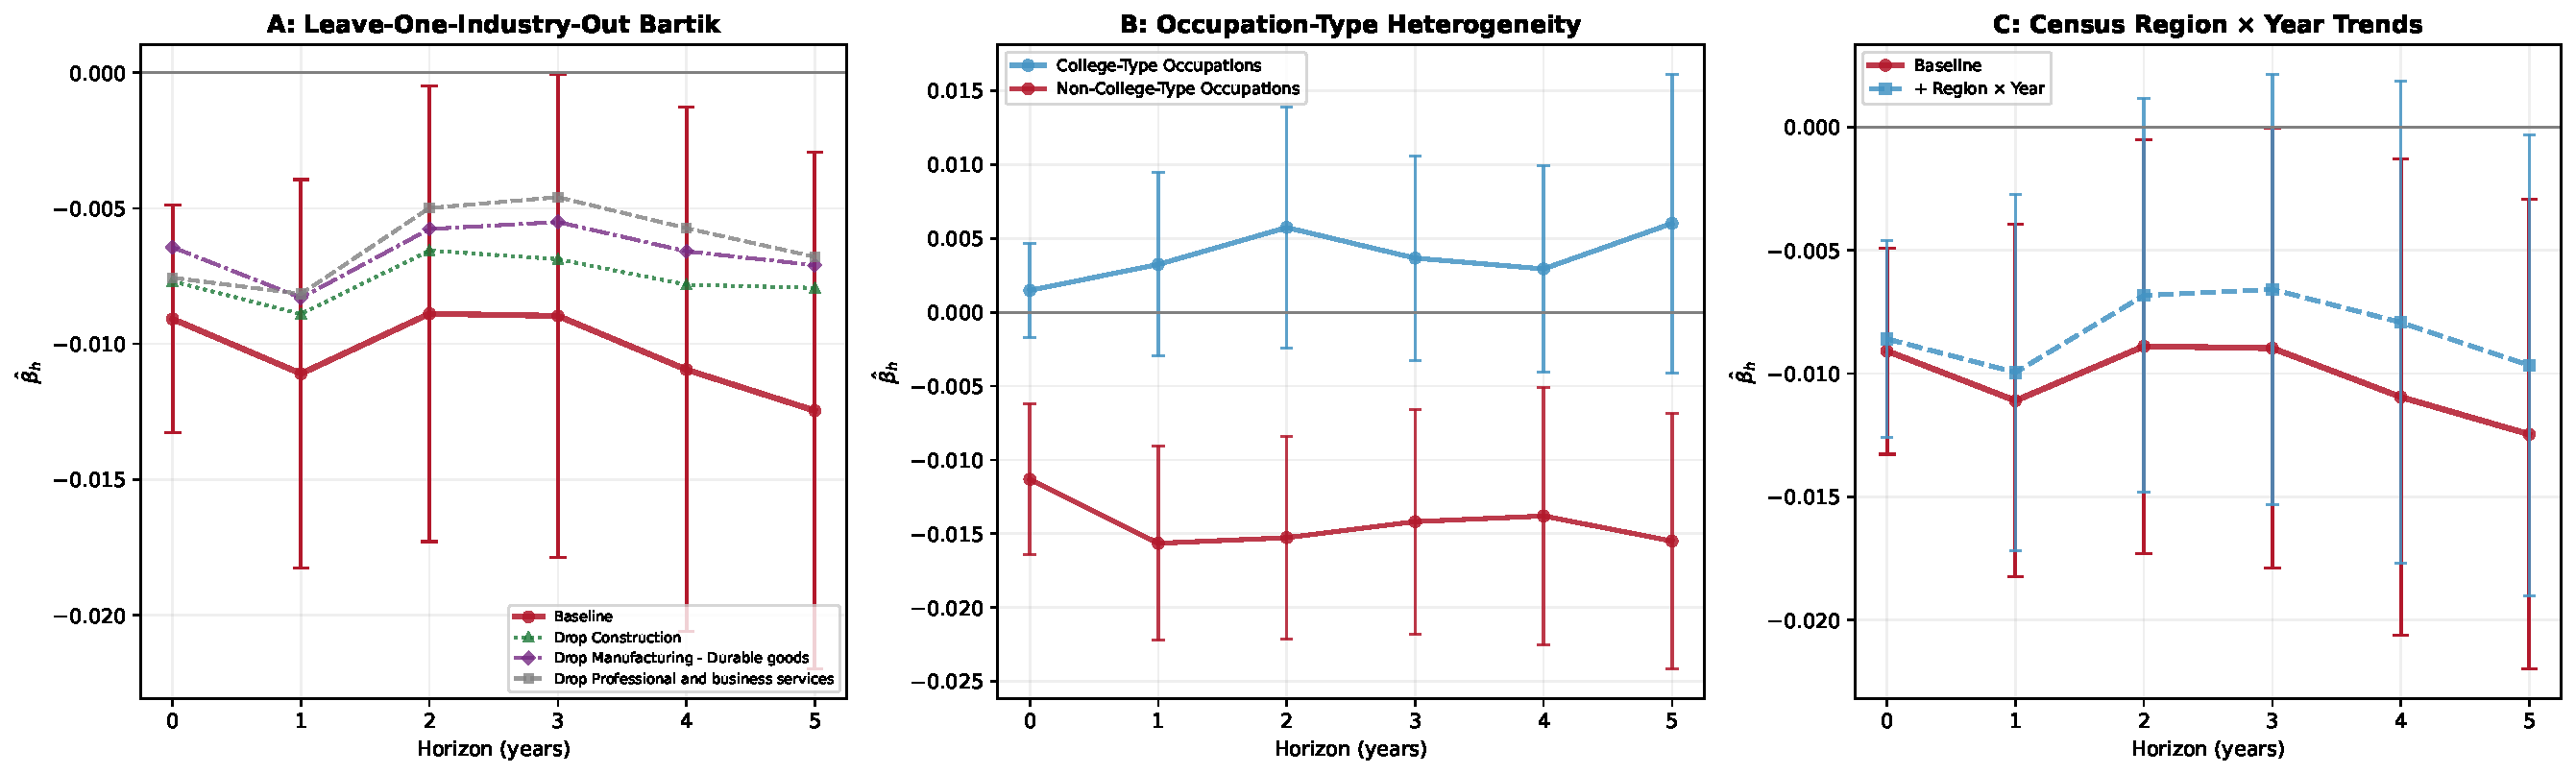
\includegraphics[width=\textwidth]{../results/robustness/fig_extensions.pdf}
	\caption{(A) Leave-one-industry-out Bartik. (B) Occupation-type heterogeneity. (C) Census region $\times$ year trends.}
	\label{fig:extensions}
\end{figure}

\begin{figure}[htbp]
	\centering
	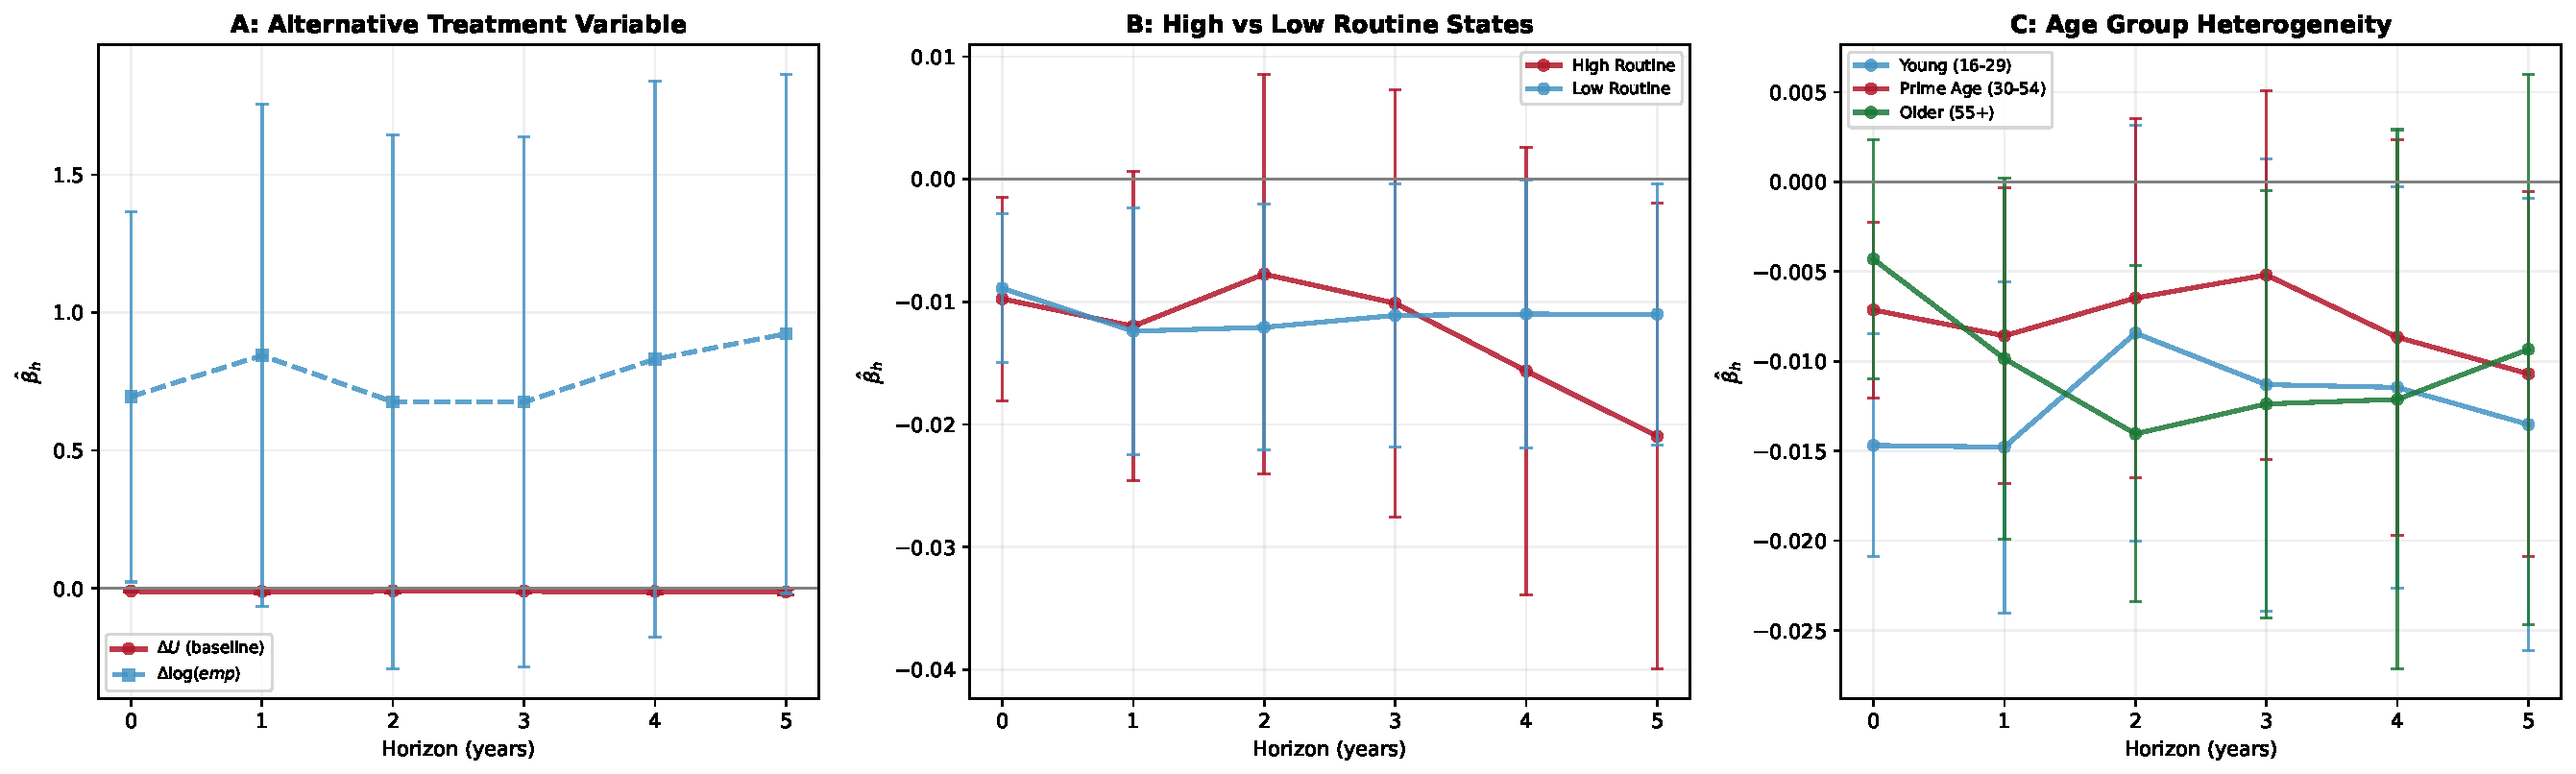
\includegraphics[width=\textwidth]{../results/robustness/fig_final_extensions.pdf}
	\caption[Final extensions]{(A) Alternative treatment: $\Delta U$ vs $\Delta \log(\text{emp})$. (B) High vs low routine states. (C) Age group heterogeneity.}
	\label{fig:final_extensions}
\end{figure}

\end{document}
